% This is the main file for the template for doctoral thesis at
% University of Zagreb, Faculty of Electrical Engineering and Computing
% in Zagreb, Croatia.
% Initial version was created in April 2013, last update was in July 2014.

% Author: Jelena Bozek, jelena.bozek@fer.hr
% Contributor: Vedran Miletic, vmiletic@inf.uniri.hr


%%%%%%%%%%%%%%%%%%%%%%%%% POSTAVKE / SETTINGS %%%%%%%%%%%%%%%%%%%%%%%%%%%%%
\documentclass[12pt,oneside, a4paper]{book}
\usepackage{etex}
\usepackage{xcolor}
\usepackage[pdftex]{graphicx}
\usepackage{rotating}
\usepackage{epsfig}
\usepackage{epstopdf}
% required for printing index
% use \index{name} in text
%\usepackage{makeidx}
%\makeindex
% required for printing nomenclature
% use \nomenclature{symbol}{description} in text
%\usepackage{nomencl}
%\makenomenclature
%\renewcommand{\nomname}{Popis oznaka}

\usepackage[T1]{fontenc}
\usepackage[utf8]{inputenc}
\usepackage{cmap}
%\usepackage[croatian]{babel}
\usepackage{ae}
\usepackage[unicode]{hyperref}
\usepackage{mathptmx}
\usepackage{amscd}
\usepackage{amssymb}
\usepackage{amsmath}
\usepackage{amsfonts}

\usepackage[left=2.5cm,right=2.5cm,top=2.5cm,bottom=2.5cm]{geometry}
\usepackage{setspace} 
\linespread{1.3}
\usepackage{fancyhdr} % setting up header and position of page numbers
\pagestyle{fancyplain}
\fancyhf{}
\lhead{\nouppercase{\fancyplain{}{\leftmark}}}
\renewcommand{\chaptermark}[1]{\markboth{#1}{}}
\rfoot{\thepage}

\usepackage{hhline}
\usepackage{enumerate}
\usepackage{delarray}
\usepackage{array}  % package for some table properties
\usepackage{tabularx} % package that allows dynamical changing table cell width
\usepackage{multirow}  % package that enables multiple rows in a table
\usepackage[bf, font=small]{caption}
\usepackage[labelfont=small, font=small]{subcaption}
\usepackage{wasysym}
\usepackage{subeqnarray}
\usepackage{aeguill}
\usepackage{pdflscape} % setting page into landscape view
\usepackage{enumitem} % for itemize lists
\setlist{nolistsep}   % setting for itemize lists

\renewcommand{\thefootnote}{\fnsymbol{footnote}}  % to get unnumbered footnotes
\renewcommand{\arraystretch}{1.5} % stretching row height

\usepackage[square, numbers, sort]{natbib} 



% Adding a dot after chapter number in TOC 
\let\savenumberline\numberline
\def\numberline#1{\savenumberline{#1.}}

% Adding dots after chapter titles to page number in TOC
\makeatletter
\renewcommand*\l@chapter[2]{%
  \ifnum \c@tocdepth >\m@ne
  \addpenalty{-\@highpenalty}%
  \vskip 1.0em \@plus\p@
  \setlength\@tempdima{1.5em}%
  \begingroup
  \parindent \z@ \rightskip \@pnumwidth
  \parfillskip -\@pnumwidth
  \leavevmode \bfseries
  \advance\leftskip\@tempdima
  \hskip -\leftskip
  #1\nobreak\normalfont\leaders\hbox{$\m@th
    \mkern \@dotsep mu\hbox{.}\mkern \@dotsep
    mu$}\hfill\nobreak\hb@xt@\@pnumwidth{\hss #2}\par
  \penalty\@highpenalty
  \endgroup
  \fi}
\makeatother

% adjust the line spacing in a matrix
\makeatletter
\renewcommand*\env@matrix[1][\arraystretch]{%
  \edef\arraystretch{#1}%
  \hskip -\arraycolsep
  \let\@ifnextchar\new@ifnextchar
  \array{*\c@MaxMatrixCols c}}
\makeatother

% remove footer (page number) from TOC, list of figures and list of tables
\AtBeginDocument{\addtocontents{toc}{\protect\thispagestyle{empty}}}
\AtBeginDocument{\addtocontents{lof}{\protect\thispagestyle{empty}}}
\AtBeginDocument{\addtocontents{lot}{\protect\thispagestyle{empty}}}


\begin{document}


%%%%%%%%%%%%%%%%%%%%%%%%%%%%%%%%%%%%%%%%%%%%%%%%%%%%%%%%%%%%%%%%%%%%%%%%%%%
\frontmatter

%%%%%%%%%%%%%%%%%%%% NASLOVNICA / FRONT COVER PAGE %%%%%%%%%%%%%%%%%%%%%%%%
\begin{titlepage}
  \fontsize{16pt}{20pt}\selectfont
  \fontfamily{phv}\fontseries{mc}\selectfont
  \newgeometry{left=3cm,right=3cm,top=3cm,bottom=2.5cm}
  \setlength{\intextsep}{0pt plus 0pt minus 0pt}

  \begin{center}
    \begin{figure}[ht!]
      \begin{center}
        \includegraphics[height=4.1184cm, width=5.94cm]{logo_unizg_eng}
      \end{center}
    \end{figure}
    \vspace{0cm}
    {FACULTY OF SCIENCE} \\
    \vspace{3cm}
    Jelena Luetić \\
    \vspace{2cm}
    {\fontsize{22pt}{22pt}\selectfont\textbf{Measurement of the cross section for associated production of a W boson and two b quarks with the CMS detector at the Large Hadron Collider}} \\
    \vspace{2cm}  
    DOCTORAL THESIS \\    
    \vfill{Zagreb, 2015.}
  \end{center}
  \restoregeometry
\end{titlepage}
%%%%%%%%%%%%%% Prva UNUTARNJA STRANICA / SECOND INNER PAGE %%%%%%%%%%%%%%%
\begin{titlepage}
  \fontsize{16pt}{20pt}\selectfont
  \fontfamily{phv}\fontseries{mc}\selectfont
  \newgeometry{left=3cm,right=3cm,top=3cm,bottom=2.5cm}
  \setlength{\intextsep}{0pt plus 0pt minus 0pt}

  \begin{center}
    \begin{figure}[ht!]
      \begin{center}
        \includegraphics[height=4.1184cm, width=5.94cm]{logo_unizg_eng}
      \end{center}
    \end{figure}		
    \vspace{0cm}
    {\fontsize{16pt}{16pt}{FACULTY OF SCIENCE}} \\
    \vspace{3cm}
    Jelena Luetić \\
    \vspace{2cm}
    {\fontsize{22pt}{22pt}\selectfont\textbf{Measurement of the cross section for associated production of a W boson and two b quarks with the CMS detector at the Large Hadron Collider}} \\
    \vspace{2cm}   
    DOCTORAL THESIS \\  
    \vspace{5cm}   % adjust this spacing if necessary
    Supervisor: Professor Vuko Brigljević, PhD \\
    \vfill{Zagreb, 2015}
  \end{center}
  \restoregeometry
\end{titlepage}
%%%%%%%%%%%%%%% Druga UNUTARNJA STRANICA / FIRST INNER PAGE %%%%%%%%%%%%%%%%
\begin{titlepage}
  \fontsize{16pt}{20pt}\selectfont
  \fontfamily{phv}\fontseries{mc}\selectfont
  \newgeometry{left=3cm,right=3cm,top=3cm,bottom=2.5cm}
  \setlength{\intextsep}{0pt plus 0pt minus 0pt}

  \begin{center}
    \begin{figure}[ht!]
      \begin{center}
        \includegraphics[height=4.1184cm, width=5.94cm]{logo_unizg2}
      \end{center}
    \end{figure}		
    \vspace{0cm}
    {PRIRODOSLOVNO MATEMATIČKI FAKULTET} \\
    \vspace{3cm}
    Jelena Luetić \\
    \vspace{2cm}
    {\fontsize{22pt}{22pt}\selectfont\textbf{Mjerenje udarnog presjeka zajedničke produkcije W bozona i para b kvarkova CMS detektorom na Velikom hadronskom sudarivaču}} \\
    \vspace{2cm}    
    DOKTORSKI RAD \\
    \vspace{5cm}    % adjust this spacing if necessary
    Mentor: Prof. dr. sc. Vuko Brigljević \\
    \vfill{Zagreb, 2015.}
  \end{center}
  \restoregeometry
\end{titlepage}



%%%%%%%%%%%%%%%%%%%%%%%%%%%%%%%%%%%%%%%%%%%%%%%%%%%%%%%%%%%%%%%%%%%%%%%%%%%
\begin{titlepage}
  \begin{minipage}{\dimexpr\textwidth-1cm}
    \vspace{3cm}
    Doktorski rad izrađen je na Sveučilištu u Zagrebu
    Prirodoslovno matematičkom fakultetu

    \vspace{1cm}
    Mentor: prof. dr. sc. Vuko Brigljević

    \vspace{1cm}
    Doktorski rad ima: XYZ stranica

    \vspace{1cm}
    Doktorski rad br.: \line(1,0){64}
  \end{minipage}
\end{titlepage}


%%%%%%%%%%%%%%%%%%%%%%%%%%%%%%%%%%%%%%%%%%%%%%%%%%%%%%%%%%%%%%%%%%%%%%%%%%%
% insert optional page with thanks or dedication
%\include{eg_thanks_dedication}



%%%%%%%%%%%%%%%%%%%%%%%%%%%%%%%%%%%%%%%%%%%%%%%%%%%%%%%%%%%%%%%%%%%%%%%%%%%
\clearpage
%%%%%%%%%%%%%%%%%%%%%%%%%%%%%%%%% TOC %%%%%%%%%%%%%%%%%%%%%%%%%%%%%%%%%%%%%
\pagestyle{empty} % remove header/footer 
\tableofcontents
\cleardoublepage % start new page

%\pagestyle{fancyplain} % puts headers/footers back on


%%%%%%%%%%%%%%%%%%%%%%%%%%%%%%%%%%%%%%%%%%%%%%%%%%%%%%%%%%%%%%%%%%%%%%%%%%%

\mainmatter % Begin numeric (1,2,3...) page numbering

\pagestyle{fancy} % Return the page headers back to the "fancy" style

% Include the chapters of the thesis as separate files from the Chapters folder
% Uncomment the lines as you write the chapters

%% Chapter 1

\chapter{Introduction} % Main chapter title

\label{Chapter1} % For referencing the chapter elsewhere, use \ref{Chapter1} 

\lhead{Chapter 1. \emph{Introduction}} % This is for the header on each page - perhaps a shortened title

% Filozofija
The standard model of particle physics tries to give an answer to the questions what is the matter made of and how does it interact. The predictions of the standard model have been thoroughly tested many times and various precision measurements were performed at different experiments. Nevertheless every time the standard model predictions were confirmed. The only missing link, the long sought Higgs boson, was found in 2012, with its properties measured in the following years thus completing the picture of elementary particles. However, standard model still leaves some unexplained phenomena, e.g. neutrino oscillations, matter-antimatter asymmetry, the existence of dark matter and dark energy, giving rise to the physics beyond standard model. The sensitivity of such processes in the high energy physics experiments strongly depends on the precise measurements of known processes. In such measurements, poorly known yields and kinematics of the known processes would lead to high uncertainties, and thus reducing the sensitivity of the experiment. 
% Zasto b kvark - QCD
\par The production of a W boson in association with a pair of b quarks (Wbb) has
been the topic of many theoretical studies and simulations. It is however still not well described due to divergences which arise in theoretical calculations, in cases where b quarks are collinear or there is a low energy massless particle irradiated. Several theoretical
approaches, implemented in different simulation packages, have been used to describe the Wbb production mechanism. A precise measurement of Wbb production will allow to
further constrain theoretical predictions in the framework of perturbative quantum chromodynamics (pQCD) and to test the validity of different theoretical models used in simulations. On the other hand, Wbb is a background to different standard model processes as well as beyond standard model searches. It is one of the main backgrounds to top quark  and Higgs boson measurements, in particular, events in which Higgs boson is produced in association with a W boson and decays to a pair of b quarks.
% Sto je pokazano
\par This thesis is focused on the measurement of the cross section of $pp\rightarrow W+bb+X$ process using the data collected during 2012 at $\sqrt{s} = 8$ TeV. The data is provided by the LArge Hadron Collider (LHC) accelerator at CERN, Geneva and collected by the Compact Muon Sollenoid (CMS). W boson is decaying either to an electron or muon, and a corresponding neutrino. The presence of a W boson is identified through the detection of an energetic, isolated lepton, i.e. lepton without any additional activity in some predefined cone around it, and a significant amount of missing energy, which indicates the presence of a neutrino. Jets in the detector are identified as a collimated spray of particles. Selected jets are required to be tagged as jets originating from b quarks. This procedure is called b-tagging and it exploits unique b quark properties to derive a single discriminator value to distinguish between b jets and jets from lighter quarks, or gluons. 
% Organizacija teze

The thesis is organized as follows. Chapter 2 shows a brief introduction to the standard model, with the emphasis on the discovery and the role of W boson and b quarks within the standard model. An overview of the phenomenology of the proton collisions at hadron colliders is shown. All the steps for the theoretical calculation of the $pp\rightarrow W+bb+X$ process are given for both, single parton scattering and double parton scattering production mechanisms. The end of the chapter summarizes all previous measurements of W boson and b quarks in the final state. Chapters 3 and 4 are focused on the description of the LHC and CMS respectively. All CMS subsystems are described and their role is explained. Chapter 5 describes the procedure for reconstruction of various physics objects, including electrons, muons and jets, and estimation of missing energy. Chapter 6 lists all data and Monte Carlo samples used. Criteria for the signal selection are described and all major backgrounds are identified. Chapter 7 describes all steps in the cross section determination, including the fitting procedure used to extract final yields, and the acceptance and efficiency estimation. In the end, the results are presented, together with the comparison to theoretical predictions. The final chapter briefly summarizes the results, and shows the prospects for the future research on this topic.

% Chapter Template

\chapter{Theoretical overview} % Main chapter title

\label{Chapter2} % Change X to a consecutive number; for referencing this chapter elsewhere, use \ref{ChapterX}

\lhead{Chapter 2. \emph{Theoretical overview}} % Change X to a consecutive number; this is for the header on each page - perhaps a shortened title

%----------------------------------------------------------------------------------------
%	SECTION 1
%----------------------------------------------------------------------------------------

\section{Standard model overview}



%-----------------------------------
%	SUBSECTION 1.2
%-----------------------------------
\subsection{Elementary particles of Standard model}

\subsubsection{b quarks}

\subsubsection{Discovery and role of W boson}


%-----------------------------------
%	SUBSECTION 1.2
%-----------------------------------
\subsection{Electroweak interactions}



%-----------------------------------
%	SUBSECTION 1.3
%-----------------------------------

\subsection{Higgs mechanism}


%----------------------------------------------------------------------------------------
%	SECTION 2
%----------------------------------------------------------------------------------------

\section{Wbb at hadron collider}

%-----------------------------------
%	SUBSECTION 2.1
%-----------------------------------

\subsection{Cross sections at hadron colliders}

\begin{figure}[htbp]
	\centering
		\includegraphics{Figures/pp_xsec.pdf}
		\rule{35em}{0.5pt}
	\caption[Proton-proton cross sections]{Standard model cross sections as a function of center of mass energy.\citep{Campbell:2006wx} }
	\label{fig:pp_xsec}
\end{figure}

%-----------------------------------
%	SUBSECTION 2.2
%-----------------------------------

\subsection{Contributions to Wbb cross section}



%----------------------------------------------------------------------------------------
%	SECTION 3
%----------------------------------------------------------------------------------------

\section{Previous measurements} 
% Chapter Template

\chapter{Large Hadron Collider} % Main chapter title

\label{Chapter3} % Change X to a consecutive number; for referencing this chapter elsewhere, use \ref{ChapterX}

\lhead{Chapter 3. \emph{Large Hadron Collider}} % Change X to a consecutive number; this is for the header on each page - perhaps a shortened title

CERN is the largest particle physics laboratory in the world, located near the city of Genava, on the French-Swiss border. It was founded in 1953 by 12 countries and today it has 21 member states. It's main function is to provide particle accelerators and infrastructure for high energy physics experiments. Current accelerator complex is a chain of smaller accelerators with increasingly higher energies of which the largest one is Large Hadron Collider (LHC) (Figure \ref{fig:LHC}). Protons accelerated in the chain are obtained by taking hydrogen atoms and stripping them of the orbiting electrons. Protons are then accelerated by a small linear accelerator Linac2 to 50 MeV and injected to PS Booster. After reaching 1.4 GeV, protons are injected to Proton Synchrotron and accelerated to 25 GeV. Next accelerators in chain are Super Proton Synchrotron (SPS) with energy of 450 GeV, and Large Hadron Collider with beam energy of 7 TeV. In addition to proton-proton collisions, LHC is also able to deliver lead-lead collisions and lead-proton collisions. 
Some of the major physics results at CERN include the discovery of neutral currents, discovery of W and Z bosons, creation of antihydrogen atom and direct observation of CP violation among others. 
In this chapter, we will briefly go through the motivation for the LHC design, building blocks of the LHC will be presented together with the accelerator performance during the past few years.   
\begin{figure}[htbp]
	\centering
		\includegraphics[width=0.8\textwidth]{Figures/LHC.jpg}
		%\rule{35em}{0.5pt}
	\caption[Schematics of Large Hadron Collider]{Schematics of Large Hadron Collider}
	\label{fig:LHC}
\end{figure}
%----------------------------------------------------------------------------------------
%	SECTION 1
%----------------------------------------------------------------------------------------

\section{Physics goals for the LHC}

The standard model of elementary particles describes nicely all known particles and interactions, however there are still some unanswered questions. One of the major question was the existence of Higgs boson which was solved in the past few years with the discovery of a new particle at 125 GeV. In order to be able to claim a discovery, all known standard model processes have to be well measured and understood. This requirement lead to many precision measurements which determined precisely cross sections, couplings, masses and other parameters within the standard model. Any deviation from standard model predictions can be an evidence for physics beyond standard model. One of the questions that remain open is the unification of fundamental forces, as it is difficult to construct a theory of gravity which would be similar to those of other fundamental interactions. One attempt to achieve this goal is the theory of supersymmetry which predicts that each particle has its heavier supersymmetric partner which according to some theories could unify all fundamental forces. If the theory of supersymmetry is correct, lightest supersymmetic particles could be found at the LHC. This could potentially solve the problem of the dark matter which could be, according to some theories, undiscovered supersymmetric particles. Also the problem of matter-antimatter asymmetry could be addressed trying to discover why is the world built only of matter. Other theories that involve extra dimensions, bound states of quarks and leptons LHC also performed lead-lead and lead-proton collisions in which a state called quark-gluon plasma is produced that resembles the conditions in the early universe. 
\par During the past few years, various models for new physics have been extensively tested, and new exclusion limits have been set. After three years of data taking at 7 and 8 TeV, and a shutdown period of two years, LHC is now almost ready to deliver collisions at record energies of 13 TeV which could hopefully show signs of new physics.        

%-----------------------------------
%	SECTION 2
%-----------------------------------

\section{Design of the LHC}

The LHC is placed inside a 27 km tunnel, which lies between 45 m and 170 m below the ground surface and previously housed LEP accelerator. Beams circulating inside the LHC, collide at four interaction points. At each of these points, a detector has been built to record the products of proton collisions. This thesis uses data collected by the CMS (Compact Muon Solenoid) detector. Other detector with the same purpose but different design is the ATLAS (A Toroidal LHC Apparatus) detector located at the opposite side of the LHC ring. These two are so called multiple purpose particle detectors, covering a large portion of spacial angle around the interaction point, and aimed towards discovering Higgs boson, supersymmetry, precision measurements etc. The other two experiments are ALICE (A Large Ion Collider Experiment) which is designed to study quark-gluon plasma from lead collisions, and LHCb (LHC Beauty) for B physics. Two other experiments TOTEM and LHCf are placed away from the interaction point to measure the products along the beam direction.
\par Magnets
\par vacuum
\par beam pipe
\par rf cavities
    

\begin{figure}[htbp]
	\centering
		\includegraphics[width=0.7\textwidth]{Figures/LHC_magnet.pdf}
		%\rule{35em}{0.5pt}
	\caption[Schematics of dipole magnets]{Schematics of Dipole magnets \cite{Evans:2008zzb}}
	\label{fig:LHC_mag}
\end{figure}

%-----------------------------------
%	SECTION 3
%-----------------------------------

\section{Performance}

Since the start of the LHC in 2009, there were three years of machine operation, which yielded many physics results among which the discovery of Higgs boson reported by ATLAS and CMS collaborations. should be highlighted. First year of operation was devoted to commissioning and understanding machine characteristics with the emphasis on safety and testing machine protection systems. In 2011 new energy and instantaneous luminosity records were reached. These numbers were increased once again in 2012 with center of mass energy going to 8 TeV.
\par High bunch intensity with 50 ns bunch spacing was used in order to get a good instantaneous luminosity performance. This came at a cost of high number of collisions in one bunch crossing (pile-up) which was in 2012 around 12 collisions, and in some cases this number went as high as 20 interactions. With the increase of instantaneous luminosity in 2012, number of pile-up interactions was on the average around 30. Besides proton-proton collisions, LHC successfully delivered lead-lead ion runs in 2010 and 2011. primarily for the ALICE experiment, but also for CMS and ATLAS. At the start of 2013. there was also a successful proton-lead run performed for the first time. 

\begin{table}[h]
\centering
  \caption{LHC performance in 2012 together with design performance \cite{Evans:2008zzb}}
  \begin{tabular}{ l  c  c }
      \hline
      \hline
      Parameter & Design value & Value in 2012 \\
      \hline
      Beam energy [TeV] & 7 & 4 \\
      Bunch spacing [ns] & 25 & 50 \\
      Number of bunches & 2808 & 1374 \\
      Protons per bunch & 1.15$\times 10^{11}$ & 1.6-1.7$\times 10^{11}$ \\
      Peak luminosity [cm$^{-2}$s$^{-1}$] & 1$\times 10^{34}$ & 7.7$\times 10^{33}$ \\
      Max. number of events per bunch crossing & 19 & $\approx 40$ \\
      Stored beam energy [MJ] & 362 & $\approx$ 140 \\
      \hline
      \hline 
  \end{tabular}
\end{table}

LHC achieved very good luminosity performance during pat years mainly because of the excellent beam quality delivered by the injectors with significantly more protons than nominal and with lower emittances. Since the LHC was capable to absorb these beams, it was chosen to continue to operate with 50 ns bunch spacing. This meant higher pile-up which had to be dealt with by the experiments. 


\begin{table}[h]
\centering
  \caption{LHC performance highlights}
  \begin{tabular}{ l  c }
      \hline
      \hline
      Max. luminosity delivered in one fill & 237 pb$^{-1}$  \\
      Max. luminosity delivered in 7 days & 1.35 fb$^{-1}$  \\
      Longest time in stable beams (2012) & 22.8 hours \\
      Longest time in stable beams over 7 days & 91.8 hours (55$\%$) \\
      \hline
      \hline 
  \end{tabular}
\end{table}

\begin{figure}[htbp]
	\centering
		\includegraphics[width=0.7\textwidth]{Figures/lumi.png}
		%\rule{35em}{0.5pt}
	\caption[Luminosity delivered to the CMS experiment]{Luminosity delivered to the CMS experiment}
	\label{fig:LHC_lumi}
\end{figure}
 
Following a two year shutdown, LHC is anticipating operations at even higher energies of 6.5 TeV and later 7 TeV. The long term plan includes even higher peak luminosities, installation of the new injector complex and later the beginning of HL-LHC era. The timeline will, of course, be highly affected by the performance and results of the next run.
\chapter{Compact Muon Solenoid} % Main chapter title

\label{Chapter4} % Change X to a consecutive number; for referencing this chapter elsewhere, use \ref{ChapterX}

\lhead{Chapter 4. \emph{Compact Muon Solenoid}} % Change X to a consecutive number; this is for the header on each page - perhaps a shortened title

Compact Muon Solenoid is a general purpose detector designed to be able to cover a wide range of physics at the LHC. It has a layered design with each layer detecting different kinds of particles and covering a large portion or the spherical angle around the interaction point. Inside a large soleonid, with a tracker and calorimeter built inside to improve the resolution of the momentum measurements. Detectors outside the solenoid are designed primarily to detect muons. 
\par This chapter is organized in subsections describing each part of the detector separately together with it's role in CMS.  

%----------------------------------------------------------------------------------------
%	SECTION 1
%----------------------------------------------------------------------------------------

\section{CMS coordinate system}

CMS uses a right-handed coordinate system with the origin in the interaction point. $z-$axis is pointing along the beam line. $x-$axis is pointing towards the center of the ring while y axis points upwards. Two angles are used when describing position inside the detector, azimuthal angle $\phi$ and polar angle $\theta$. $\phi$ angle lies in $x-y$ plane with range $[-\pi,\pi]$

%----------------------------------------------------------------------------------------
%	SECTION 2
%----------------------------------------------------------------------------------------

\section{Inner tracker system}


%-----------------------------------
%	SUBSECTION 2.1
%-----------------------------------
\subsection{Pixel Detector}


%-----------------------------------
%	SUBSECTION 2.2
%-----------------------------------

\subsection{Strip detector}

%----------------------------------------------------------------------------------------
%	SECTION 3
%----------------------------------------------------------------------------------------

\section{Electromagnetic calorimeter}



%----------------------------------------------------------------------------------------
%	SECTION 4
%----------------------------------------------------------------------------------------

\section{Hadronic calorimeter}


%----------------------------------------------------------------------------------------
%	SECTION 5
%----------------------------------------------------------------------------------------

\section{Solenoid}


%----------------------------------------------------------------------------------------
%	SECTION 6
%----------------------------------------------------------------------------------------

\section{Muon chambers}

%----------------------------------------------------------------------------------------
%	SECTION 7
%----------------------------------------------------------------------------------------

\section{Trigger}

%----------------------------------------------------------------------------------------
%	SECTION 8
%----------------------------------------------------------------------------------------

\section{Data acquisition system} 
\chapter{Physics objects definitions} % Main chapter title

\label{Chapter5} % Change X to a consecutive number; for referencing this chapter elsewhere, use \ref{ChapterX}

\lhead{Chapter 5. \emph{Physics object definitions}} % Change X to a consecutive number; this is for the header on each page - perhaps a shortened title

The CMS detector is designed to efficiently reconstruct and identify interesting physics objects. The reconstruction procedure which takes as input the signals from all subdetectors and combines them to get physics objects is called \textit{particle flow} \cite{CMS:2009nxa}. This algorithm classifies all the objects into one of the following categories: charged hadrons, neutral hadrons, photons, electrons and muons. These are built from reconstructed tracks in the inner tracking system, energy deposits in the calorimeters and signals in the muon chambers, which are all combined to create a global event description. Additionally, a set of requirements is imposed on both input signals and reconstructed object in order to minimize the misidentification, e.g wrongly identifying electron as a jet. 
\par The Following sections show electron and muon reconstruction procedures and identification criteria. Jet reconstruction procedure is then described together with necessary jet corrections and b-tagging algorithms. After the reconstruction of all other objects, missing transverse energy is computed.

%----------------------------------------------------------------------------------------
%	SECTION 1
%----------------------------------------------------------------------------------------

\section{Electrons}

Electrons in CMS are detected as a tracks in tracking system and an energy deposit in the electromagnetic calorimeter. Two different algorithms are used for electron reconstruction, \textit{tracker driven} seeding which is more suitable for low $p_T$ electrons and electrons inside jets and \textit{ECAL driven} seeding optimized for high $p_T$ isolated electrons. Both approaches take electromagnetic crystals with deposited energy and join them into \textit{clusters}. This process begins by identifying the cryistal with the highest energy deposit which becomes the seed for the cluster. An electron passing through the detector bends due to the magnetic field and interacts with the detector material emitting \textit{bremsstrahlung} photons. ECAL energy deposits from these photons are spread in $\phi$ direction in a very narrow $\eta$ range and combined with the existing cluster forming a \textit{supercluster}. Trajectories are reconstructed using modeling of electron energy loss in the detector material and fitted with a Gaussian Sum Filter(GSF) \cite{2005JPhG31N9A}.
\par The two approaches differ in the way they match ECAL superclusters and reconstructed tracks. Tracker driven algorithms use track from the tracking system and try to match it with the supercluster in the ECAL, while ECAL driven algorithms start from the superclusters.
Each electron candidate has to pass various quality criteria in order to maximize the probability of identifying the electron coming from the hard interaction, and reject electrons from jets or conversions. These selection criteria can be divided into three categories: identification, isolation and conversion rejection. Details on electron reconstruction and performance can be found in \cite{CMS:2010bta}.

%-----------------------------------
%	SUBSECTION 1.1
%-----------------------------------
\subsubsection*{Electron identification}
\label{sec:eleID}

The electron identification procedure first focuses on good matching between reconstructed track and supercluster, by imposing cuts on spatial distance $\Delta \eta$ and $\Delta \phi$ between the two. These variables are computed as absolute $\eta$ and $\phi$ distance between the supercluster and electron track extrapolated to the ECAL surface. Additionally, a cut is imposed on $\sigma_{i\eta i\eta}$ which is a measure of a shower shape spread in $\eta$ direction. This variable discriminates between energy deposits coming from electrons and photons, which are narrow, and jets, which are wide. Shower shape is defined as:
\begin{equation}
\sigma_{i\eta i\eta} = \sqrt{\frac{\sum_{i}^{5\times 5} w_i(\eta_i-\eta_{seed})^2\times \Delta \eta^2_{xtal} }{\sum_{i}^{5\times 5}}}
\end{equation}
where $i$ runs over all crystals in $5\times5$ block around the supercluster seed, $\eta_i-\eta_{seed}$ is the distance in number of crystals in $\eta$ direction between $i$-th crystal in supercluster and the seed crystal and $\Delta \eta_{xtal}$ is the average width of a single crystal. Each crystal is given a weight defined as $w_i=max(0,4.7+ln(E_i/E_{5\times5}))$, where $E_i$ is a single crystal energy, and $E_{5\times 5}$ is the sum of energy deposits inside a 5$\times$5 crystal block. 
Additional cut on the ratio between the energy deposits in the hadronic and electromagnetic calorimeter for electrons is used to discard the electron candidates with significant hadron activity.
\par Electrons coming from photon conversions are rejected by requiring a hit in every layer of the inner tracking system. Additionally, for each electron track a fit is performed trying to combine it with another electron track under the hypothesis that both electrons originate from a converted photon. Electron is selected only if this probability is sufficiently small. Electron compatibility with the primary vertex is estimated by looking at the impact parameters in both $xy$ and $z$ planes. Due to the gap in the electromagnetic calorimeter in 1.4442 $< |\eta| <$ 1.566, all electrons which have a supercluster position reconstructed in this range are rejected. A full list of identification criteria is summarized in Table \ref{tab:eleID}.
 \begin{table}[h]
\centering
  \caption{Summary of electron identification criteria used in this analysis.}
  \label{tab:eleID}
  \begin{tabular}{ l  c c}
      \hline
      \hline
      	Variable & Barrel & Endcap \\
      	\hline
    		$\Delta\eta$ $<$ &  0.004 & 0.005 \\
     	$\Delta\phi$ $<$ &  0.03 & 0.02 \\
     	$\sigma_{i\eta i\eta}$ $<$ & 0.01 & 0.03 \\
		$H/E$ $<$ & 0.12 & 0.10 \\
		$d_{xy}$ $<$ & 0.02 cm & 0.02 cm \\
		$d_{z}$ $<$  & 0.1 cm & 0.1 cm \\
		$(1/E - 1/p)$ $<$ & 0.05 & 0.05\\
		Missing hits  & 0 & 1 \\
		Vertex Fit Probability & $10^{-6}$ & $10^{-6}$ \\    	

      \hline
      \hline 
  \end{tabular}
\end{table}


%----------------------------------------------------------------------------------------
%	SECTION 2
%----------------------------------------------------------------------------------------

\section{Muons}

Muons in CMS are reconstructed by combining a reconstructed track inside the tracker(\textit{tracker track}) and a track in muon chambers (\textit{standalone muon track}). Individual track segments in the muon chambers are fitted using a Kalman fitter technique \cite{Fruhwirth1987444}  in order to obtain a standalone muon track. As for electrons, two approaches are used for combining track from tracker and standalone track. 
\par \textit{Global muon reconstruction} approach uses a standalone muon track in the muon chambers and tries to find a matching tracker track by combining parameters of the two tracks by projecting it to the common surface. This \textit{outside-in} approach uses Kalman fitter technique to combine these two objects in an object called \textit{global muon}. Muon momentum is then determined from this global muon track using all available systems which shows improved precision in comparison to other approaches.  
\par The second approach for muon reconstruction is \textit{tracker muon reconstruction} which starts from tracks inside the tracker with $p_T>0.5$ GeV/c and total momentum $p>2.5$ GeV/c as potential muon candidates. Extrapolation is than performed to the muon chambers taking into account the magnetic field, Coulomb scattering in the material and other energy losses. \textit{Tracker moun} is found if at least one muon segment matches the extrapolated track. The efficiency of the \textit{Tracker muon} reconstruction is higher for low energy muons than the efficiency for the global muons, because only a single muon segment in the muon chambers is required. For high energy muons where there are more segments inside muon chambers, \textit{global muon} algorithm is designed to have high efficiency. Detailed muon reconstruction procedure is shown in \cite{2012JInst7P0002T}.    

%-----------------------------------
%	SUBSECTION 2.1
%-----------------------------------

\subsubsection*{Muon identification}
\label{sec:muID}

In this analysis \textit{particle flow} muon identification selection is applied to the \textit{global muons}. Selection is applied in order to minimize misidentification of charged hadrons as muons, maximize the efficiency of muon identification inside jets and ensure good momentum measurement. Muons used in the analysis have $|\eta|<2.1$ and transverse momentum $p_T>30$ GeV with more than 5 hits in the inner tracker system and at least one hit in pixel detector. At least one good muon chamber hit is required and the \textit{global muon} track fit is required to have $\chi^2/ndof<10$. At least two segments in two different muon stations should be matched to a track in order to suppress muons from in-flight decays. Cosmic muons are rejected by applying cuts on the impact parameter with respect to the primary vertex of $|d_{xy}|<$0.2 cm and $|d_z|<$ 0.5 cm. Muon identification criteria are summarized in Table \ref{tab:muID}.

  \begin{table}[h]
\centering
  \caption{A summary of muon identification criteria.}
  \label{tab:muID}
  \begin{tabular}{ l  c c}
      \hline
      \hline
      	Variable & Requirement \\
      	\hline
    		number of pixel hits $>$ &  0 \\
     	number of inner tracker hits $>$ &  5 \\
     	$\chi^2/ndof$ $<$ & 10 \\
		number of muon hits $>$ & 0  \\
		chambers with matched segments $>$ & 1  \\		
		$d_{xy}$ $<$ & 0.2 cm \\
		$d_{z}$ $<$  & 0.5 cm \\
      \hline
      \hline 
  \end{tabular}
\end{table}
 

%-----------------------------------
%	SUBSECTION 2.2
%-----------------------------------

\section{Lepton isolation}
Leptons from W decays are in general expected to be well isolated from other particles in the final state. The degree of isolation is calculated using \textit{particle flow} approach by summing the transverse momenta contributions of particles around the lepton inside a specific cone. All charged particles are considered as well as photons and neutral hadrons with $p_T>$0.5 GeV. The cone used for determination of energy deposits is defined as $\Delta R = \sqrt{\Delta \phi^2+ \Delta \eta^2}$ around the lepton axis and isolation measure is defined as:
\begin{equation}
I_{PF}^{rel} = \frac{\sum p_T^{charged} + max(0, \sum E_T^{\gamma}+\sum E_T^{neutral}-0.5\sum E_T^{PU})}{p_T^l}
\end{equation}
where $\sum p_T^{charged}$ is the sum of the momenta of charged hadrons and $E_T^{\gamma} $ and $E_T^{neutral}$ are the sums of photon and neutral hadron momenta. $E_T^{PU}$ is the sum of the pile-up transverse energies from neutral particles and is calculated as a sum of track transverse momenta not coming from the primary vertex inside the isolation cone. This is multiplied by the factor of 0.5, which corresponds approximately to the ratio of neutral to charged hadron production in the hadronization process of pile-up interactions. Selected muons are required to pass isolation cut $I_{rel}^{PF}<0.12$. On the other hand, if there is a requirement that there be no leptons in the event, the isolation cut is $I_{PF}^{rel}<0.2$. Electron isolation is computed in the same way with cut of $I_{rel}^{PF}<0.1$ for selected electrons and $I_{rel}^{PF}<0.15$ for vetoed additional electrons.


%----------------------------------------------------------------------------------------
%	SECTION 3
%----------------------------------------------------------------------------------------

\section{Jets}

In high energy physics, a jet is a collimated group of hadrons which emerges as a result of quark or gluon fragmentation and hadronization process. Hadrons reconstructed in a particle detector need to be combined in order to form a jet and give information about the initial parton. A set of rules has to be created which define how to group particles and how to assign momentum to the jet. Usually this is done by summing the four-momentum of each particle in a jet.

%-----------------------------------
%	SUBSECTION 3.1
%-----------------------------------

\subsection{Jet algorithms}

Jet algorithms take into account the distance between particles and define rules to determine which particle belongs to what jet. The Same jet algorithms should be applicable to both, experimental data and theoretical calculation.  Other important properties of jet algorithms are \textit{infrared safety} and \textit{collinear safety} which means if an event is modified by addition of soft emission of collinear splitting, the final number of hard jets will remain unchanged. These two properties together are called \textit{IRC safety}. IRC unsafe jet algorithms may break the cancellation of divergences by yielding one set of jets for tree-level splitting while loop diagrams lead to another, as shown if figure \ref{fig:jet_unsafe}, giving infinite cross-sections in the full calculations. Jet definitions, jet relation to partons and an overview of different jet algorithms are summarized in \cite{Salam:2009jx}.
\begin{figure}[htbp]
	\centering
		\includegraphics[width=0.8\textwidth]{Figures/jet_unsafe2.pdf}
		%\rule{35em}{0.5pt}
	\caption[An example of configuration of IRC unsafe jet algorithm.]{Configuration showing IC  unsafety with W boson and two partons. Adding a soft gluon causes two jets to be reconstructed as one. \cite{Salam:2009jx}}
	\label{fig:jet_unsafe}
\end{figure}

\par There are two types of jet algorithms which are most commonly used: \textit{cone algorithms} and \textit{sequential recombination algorithms}. In the case of \textit{cone algorithms}, a jet is defined as a set of particles inside a stable cone around their center of mass. Most popular cone algorithm is \textit{iterative cones} (IC) where a seed particle is chosen and momenta of all particles around that initial particle inside a cone of radius $R$ are summed. After adding each new particle to the sum, the direction of the new sum is taken as a seed direction, and the procedure repeats until the direction of the resulting cone is stable. Particles inside the cone are than removed from the list of available particles and the procedure repeats. This approach is not IRC safe given that nearly collinear splitting of the hardest particle in the event can be reconstructed as two jets. In that case, a less energetic, particle, pointing in another direction, can become the hardest particle in the event, yielding different set of jets. Cone algorithms can be IRC safe using a \textit{seedless cone} (SC) algorithm where all stable cone solutions are identified at once. However this approach is very time consuming even for small number of particles and thus very impractical to use.
In the \textit{sequential recombination algorithms} at hadron colliders two longitudinally invariant distances are introduced: $d_{ij}$ which is the distance between each pair of particles and $d_{iB}$ which is the particle-beam distance. These distances are defined as: 
\begin{equation}
d_{ij} = min(k_{T,i}^{2p},k_{T,j}^{2p}) \frac{\Delta R_{ij}^2}{R^2}
\end{equation}
\begin{equation}
d_{iB}=k_{T,i}^{2p}
\end{equation}
where $\Delta R_{ij}$ denotes the distance in the $\eta -\phi$ plane and is computed as $$\Delta R_{ij}^2 = (\eta_i-\eta_j)^2+(\phi_i-\phi_j)^2.$$ $k_T$ is transverse momentum of the particle, $R$ is an angular cut-off similar to the one in \textit{cone algorithms},  and $p$ defines which particles are clustered first and is described below. Both $R$ and $p$ are free parameters of the algorithm. The algorithm is applied using the following approach: distances $d_{ij}$ between each pair of particles, and $d_iB$ for each particle are computed and minimal value is found. If $d_{ij}$ is the smallest value, particles $i$ and $j$ are combined, and treated as a new particle in the next iteration of the algorithm. In case of $d_{iB}$ being the smallest, $i$ is declared to be the final jet and is removed from the list of particles. The procedure continues until there are no more particles in the list.
\begin{figure}[htbp]
	\centering
		\includegraphics[width=0.9\textwidth]{Figures/diff_algos.pdf}
		%\rule{35em}{0.5pt}
	\caption[Clustering particles into jets with different algorithms.]{Clustering same set of reconstructed particles into jets using different jet algorithms. \cite{Salam:2009jx}}
	\label{fig:jetAlgos}
\end{figure}
\par The parameter $p$ defines which particles are clustered first thus defining the type of algorithm. The $k_T$ algorithm uses $p=1$, clustering soft particles first. This results in irregularly shaped jets, as shown in figure \ref{fig:jetAlgos}, which are sensitive to radiation in the event and difficult to calibrate. The \textit{Cambridge-Aachen} algorithm (CA) uses $p=0$ thus relying only on angular distribution of the input particles. This approach is particularly useful for jet substructure analysis and is less sensitive to radiation. The algorithm used in this analysis is anti-$k_T$ algorithm where $p=-1$ clusterizing the hardest particles first \cite{Cacciari:2008gp}. Anti-$k_T$ is an IRC safe algorithm and results with jets that are circular in shape because they are not affected by the softer components of the jet.       


%-----------------------------------
%	SUBSECTION 3.2
%-----------------------------------

\subsection{Jet corrections}
\label{sec:jetCorr}

Various measurements during the commissioning phase of the CMS detector showed that measured jet energy at detector level in general doesn't correspond to the energy of the originating particle. A jet calibration procedure is introduced to compensate for the nonlinear response of the calorimeters. This is done using a factorized approach where corrections on each level of correction are determined separately as described in \cite{Chatrchyan:2011ds}. The final corrected jet momentum is obtained from measured uncorrected transverse momentum $p^{raw}$ according to:
\begin{equation}
p^{corr} =  C_{res}(p_T'',\eta)\times  C_{abs}(p'_T) \times C_{rel}(\eta) \times C_{offset}(p_T^{raw},\eta)\times p^{raw}
\end{equation}  
Correction factors correspond to the following:
\begin{itemize}
\item The offset correction $C_{offset}$ compensates for energy contributions arising from pile-up events or instrumental noise. The offset is determined in dependence of pseudorapidity and jet area $p_T$ density which is described in detail in \cite{Cacciari2008119}.
\item The relative correction $C_{rel}$ aims at flattening the jet energy scale in pseudorapidity. The correction is determined from simulated QCD multijet events, adjusting the jet scale in all $\eta$ regions to one of the jets in $|\eta|<1.3$ without changing the absolute scale.
\item Absolute correction $C_{abs}$ flattens the jet scale in $p_T$. This correction is also determined from QCD multijet events as the inverse of average response at some fixed generated jet transverse momentum.
\item The residual correction $C_{res}$ is applied only to data in order to account for possible residual differences between data and simulation after applying absolute and relative corrections. These corrections are derived using events with momentum balance in the transverse plane, like dijet events or $Z/\gamma$ + jet events.
\end{itemize}   
$C_{offset}$ and calibration factors $C_{rel}$ and $C_{abs}$ are applied to both data and simulation and $C_{res}$ is applied only to data. Corrections are applied sequentially, in a fixed order such that $p_T' = C_{offset} \times C_{rel}(\eta) \times p^{raw}$ , and $p_T'' = C_{abs}(p'_T) \times C_{rel}(\eta) \times C_{offset}(p_T^{raw},\eta)\times p^{raw}$. Correction factors used in this analysis can be found in \cite{CMS-DP-2013-033}.
\par The total jet correction for a fixed jet $p_T$ as a function of pseudorapidity is shown in figure \ref{fig:tot_corr_eta}. The total jet correction for a fixed jet pseudorapidity as a function of transverse momentum is shown in figure \ref{fig:tot_corr_pt}. It is shown that jet energy correction factors for PF jets and JPT jets are relatively stable between 1 and 1.2 across wide $p_T$ and $\eta$ range. The total uncertainties to the jet energy corrections as a function of jet transverse momentum are shown in figure \ref{fig:tot_corr_err}.
\begin{figure}[htbp]
	\centering
		\includegraphics[width=0.9\textwidth]{Figures/jet_tot_corr_eta.pdf}
		%\rule{35em}{0.5pt}
	\caption[Total jet energy correction as a function of pseudorapidity of two different jet $p_T$ values.]{Total jet energy correction as a function of pseudorapidity of two different jet $p_T$ values. Corrections are shown for all three types of jets, calo, JPT and PF jets. Bands indicate corresponding uncertainty.\cite{Chatrchyan:2011ds}}
	\label{fig:tot_corr_eta}
\end{figure}

\begin{figure}[htbp]
	\centering
		\includegraphics[width=0.9\textwidth]{Figures/jet_tot_corr_pt.pdf}
		%\rule{35em}{0.5pt}
	\caption[Total jet energy correction as a function of transverse momentum for four different $\eta$ values.]{Total jet energy correction as a function of transverse momentum for four different $\eta$ values. Corrections are shown for all three types of jets, calo, JPT and PF jets. Bands indicate corresponding uncertainty.\cite{Chatrchyan:2011ds}}
	\label{fig:tot_corr_pt}
\end{figure}

\begin{figure}[htbp]
	\centering
		\includegraphics[width=0.9\textwidth]{Figures/jet_unc_err.pdf}
		%\rule{35em}{0.5pt}
	\caption{Total jet uncertainty and contribution from different sources in jet $p_T$ and $\eta$ \cite{CMS-DP-2013-033}}
	\label{fig:tot_corr_err}
\end{figure}

%-----------------------------------
%	SUBSECTION 3.3
%-----------------------------------

\subsection{Jet identification}
\label{sec:jetID}
This analysis uses the anti-$k_T$ algorithm with cone size $R=0.5$. Jet algorithm implementation is done in the FASTJET package \cite{Cacciari:2011ma}. Depending on which signals the algorithm is applied to, there are different kinds of jets: calo jets (calorimeter deposits used), jet-plus-track jets (calorimeter deposits complemented with tracker information) and most widely used \textit{particle flow} jets (PF). These jets are clustered from particle flow objects identified with the PF algorithm, thus using the information not only from HCAL, but also from the tracking system and ECAL, which result in much better resolution. Only the neutral fraction of  jets is measured with HCAL alone which makes about 15$\%$ of the total jet composition. PF jets show excellent performance and are the default jets for most CMS analyses. Pile-up information is also taken into account by removing charged hadrons originating from pile-up vertices from the list of particles available for the jet clusterization. This procedure is called \textit{charged hadron subtraction}. Some additional cuts to the jet composition are applied in order to ensure good jet identification. All jet identification criteria are summarized in the table \ref{tab:jetID}.  
  \begin{table}[h]
\centering
  \caption{A summary of jet identification criteria.}
  \label{tab:jetID}
  \begin{tabular}{ l  c c}
      \hline
      \hline
      	Variable & Requirement \\
      	\hline
    		Neutral hadron fraction & $<$ 0.99  \\
     	Neutral EM fraction & $<$ 0.99 \\
     	Number of Constituents & $>$ 1 \\		
		\hline
		Additional cuts for $|\eta|<2.4$ \\
		\hline
		Charged hadron fraction & $>$ 0 \\ 
		Charged multiplicity & $>$ 0 \\
		Charged EM fraction & $<$ 0.99 \\
      \hline
      \hline 
  \end{tabular}
\end{table}

%-----------------------------------
%	SUBSECTION 3.4
%-----------------------------------

\subsection{Jets from b quarks}
\label{sec:btagging}

The unique properties of the bottom quark can be used to identify hadronic jets originating from b quarks, which are usually referred to as b-jets. The long lifetime of B hadrons is a consequence of weak force decay which results in the displacement of their decay vertices by few millimeters at the LHC energies. These hadrons have relatively large masses and daughter particles with hard momentum spectra. The process of b-jet identification is called $b-tagging$. It takes one or more variables and produces a single discriminant value for each jet. This value shows how much the observed jet looks like a b-jet. There are several \textit{b-tagging} algorithms in use at CMS which are described in detail in \cite{Chatrchyan:2012jua} and the following were used in the 2012 data analysis:
\begin{itemize}
	\item \textit{Track counting}(TC) - The discriminant value is the impact parameter significance which is calculated as impact parameter value divided by the respective impact parameter uncertainty. Impact parameter significance values are sorted in the decreasing order. Depending on whether second or third value is chosen, the algorithm is denoted as high efficiency or high purity. 
	\item \textit{Jet Probability}(JP) - This algorithm combines information from several tracks inside a jet by computing a likelihood that all tracks originate from the primary vertex.  
	\item \textit{Combined secondary vertex}(CSV) - This is the most efficient \textit{b-tagging} algorithm currently used at CMS. Both secondary vertex and track related information are combined to build a CSV discriminator. It shows high efficiency even when no good secondary vertex can be reconstructed. Some of the variables used in CSV algorithm are flight distance, vertex mass, impact parameter significance, track multiplicity at the vertex and track multiplicity in a jet. The distribution of CSV discriminator is shown in figure \ref{fig:csv}.
\end{itemize}
\begin{figure}[ht]
	\includegraphics[width=\textwidth]{Figures/b-tag_csv.pdf}
	\caption{Combined secondary vertex discriminator for multijet QCD sample (left) and tt enriched sample(right)\cite{CMS:2013vea}}
	\label{fig:csv}
\end{figure}
For each non-b-jet there is a chance that it would be identified as b-jet. Based on this misidentification rate, three operating points have been defined for the discriminant value: loose, medium and tight. For an average jet of 80 GeV, these values correspond to misidentification rates of 10\%, 1\% and 0.1\% respectively. Misidentification probabilities as a function of b-jet efficiency for several algorithms are shown in figure \ref{fig:misID}. 
\begin{figure}[ht]
\centering
	\includegraphics[width=0.6\textwidth]{Figures/MisID_CSVM.pdf}
	\caption{Combined secondary vertex misidentification probability for data and MC for medium working point.\cite{CMS:2013vea}}
	\label{fig:misID}
\end{figure}



%----------------------------------------------------------------------------------------
%	SECTION 4
%----------------------------------------------------------------------------------------

\section{Missing transverse energy}

Missing transverse momentum is the imbalance in the vectorial sum of transverse momenta of all measured particles. Momentum conservation dictates that the imbalance arises from weakly interacting neutral particles such as neutrinos. Missing transverse energy is the magnitude of the missing transverse momentum and is calculated as:
\begin{equation}
E_T^{miss}= |-\sum_{i} \vec{p}_i|
\end{equation}
where $i$ goes over all visible particles. Measurement of the missing transverse energy relies on the good measurement of all other particles in the event and as such is very sensitive to detector inefficiencies, particle missmeasurements, limited acceptance of the detector, cosmic-ray particles, all of which can cause artificial missing energy. There are several approaches to determine $E_T^{miss}$. In this analysis, particle flow technique is used which tries to identify each particle in the event by combining the information from all subdetectors and gives the best missing energy resolution.\cite{CMS-PAS-PFT-09-001,Chatrchyan:2011tn} Several corrections are applied to the $E_T^{miss}$ which correct for the possible bias in the missing energy measurement:
\begin{itemize}
\item Type-I correction: propagates jet energy corrections described in Section \ref{sec:jetCorr} to missing energy. This correction replaces the missing energy calculated by summing uncorrected transverse momenta of particles in a jet by transverse momentum of a jet to which JEC were applied.
\item xy-shift correction: aimes at correcting the observed missing energy $\phi$ modulation. True missing energy distribution is expected not to depend on $\phi$ because of the rotational symmetry of collisions around the beam axis. The possible cause for such modulation  include unisotropic detector response, detector misalignment, the displacement of the beam spot. The amplitude of the modulation is observed to increase with the number of pile-up interactions so this correction can be seen as mitigation for the pile-up effects.
\end{itemize}
Missing transverse energy, together with the reconstructed muon or electron, is used to construct W boson candidates. Transverse mass distribution particularly useful in the case of a decay into two particles, when one particle cannot be detected directly but is only indicated by missing transverse energy. If the daughter particles are massless, transverse mass is described with:   
\begin{equation}
M_T=\sqrt{2p_T^{lepton}E_T^{miss}(1-cos\Delta \phi)}.
\end{equation}



 
% Chapter Template

\chapter{Event selection and analysis strategy} % Main chapter title

\label{Chapter6} % Change X to a consecutive number; for referencing this chapter elsewhere, use \ref{ChapterX}

\lhead{Chapter 6. \emph{Event selection and analysis strategy}} % Change X to a consecutive number; this is for the header on each page - perhaps a shortened title

%%----------------------------------------------------------------------------------------
%%	SECTION 1
%%----------------------------------------------------------------------------------------
%
%\section{Analysis strategy}
%
%
%%-----------------------------------
%%	SUBSECTION 1
%%-----------------------------------
%\subsection{Subsection 1}
%
%
%
%%-----------------------------------
%%	SUBSECTION 2
%%-----------------------------------
%
%\subsection{Subsection 2}
%
%
%%----------------------------------------------------------------------------------------
%%	SECTION 2
%%----------------------------------------------------------------------------------------
%
%\section{Background estimation}

Signal events are characterized by presence of a W boson and two jets which have been tagged as comming from b quarks.
Candidates for a W boson are identified as isolated muons or electron and significant missing energy.
Jets are identified as particle flow objects clustered with anti-$k_T$ alghorithm with a cone size of $0.5$.
Standard jet energy corrections and resolution smearing procedures prescribed by the Jet POG are applied.
Combined secondary vertex (CSV) alghoritm is then used to identify jets arising from fragmentation and hadronization of b-quarks.
This algohithm combines in an optimal way information about track impact parameters and identified secondary vertices
within the jet even when full vertex information is not available.
Isolated leptons not arising from W decays are not expected, and additional jet activity is minimal.

\subsection{Signal extraction}
Signal event selection is described in the Signal selection section.
For each of the major backgrounds a separate control region is defined in order to verify Monte Carlo normalizations.

The dominant backgrounds encountered in this analysis arise from few sources:
\begin{itemize}
        \item {\textbf{Top quarks:}} production of $t\bar{t}$ pairs and single top represent a challenging background at the LHC because of their relatively large production cross sections.
$t\bar{t}$ events are largely reduced by requiring an additional jet veto. Single top events are more difficult to reject relative to signal using just topological cuts,
but production cross-section is smaller resulting in a smaller contribution in the final distributions.
        \item {\textbf{W + light and c jets:}} contribution from this source of backgroung is largely reduced by applying b-tag requirement to selected jets.
        \item {\textbf{Drell-Yan:}} contribution from this process is largely reduced by requiring only one islated lepton in the final state.
        \item {\textbf{Dibosons(WW, WZ, ZZ):}} contribution from this type of background in case where one boson decays leptonicaly
and the other decays to jets  is indistinguishable from the signal events apart from the peak in the invariant mass distribution of two jets.
\end{itemize}

For this test $t\bar{t}$ multijet control region is used which is defined to be same as signal region, but requiring additional jet activity.



\subsection{Systematics}

The primary physics result described in this note is the cross section for production of a W boson and two b
jets. Systematic uncertainties on the expected signal and background yields and shapes affect
the final result. For a given sistematic variation, a new set of signal and background templates was created which may differ both in shape and normalization from the original template.  These shape variations are included in the final fit. Several sources of systematic variations have been considered:

\begin{itemize}
        \item{\textbf{Luminosity:}}
        an uncertainty of 2.2\% for luminosity measurement during 2012 datataking.
        \item{\textbf{Jet energy scale:}}
        the jet energy scale for each jet is varied within one standard deviation based on $p_T$ and $\eta$, and the efficiency of the analysis selection is recomputed to assess the systematic variation on the normalization and shape of the signal and all background components.
        \item{\textbf{Jet energy resolution:}}
        we smear the energy resolution for each jet using the Jet- MET prescription as our default, and then modified signal and background templates are created in which jet energy is smeared by $\pm 1 \sigma$ taken from JetMET POG.
        \item{\textbf{Lepton energy scale:}}
        muon and electron trigger, reconstruction, and identification ef-ficiencies are determined in data using the standard tag-and-probe technique with Z bosons. The systematic uncertainty is evaluated by varying lepton energy scale for each lepton within one standard deviation taken from POG.
        \item{\textbf{Unclustered missing energy:}}
        we follow the suggested procedure from the JetMET POG to determine the systematic uncertainty on the calibration of unclustered MET (missing energy associated with particles not clustered into jets).
        \item{\textbf{MC samples normalizations:}}
        the finite size of the signal and background MC samples are included in the normalization uncertainties. Normalizations are also allowed to vary within the uncertainties of measured Standard model cross-sections.(cite all sources)
        \item{\textbf{Jet b-tagging:}}
        official b-tagging scale factors are applied consistently to jets in signal and background events.
\end{itemize}

Contributions from different sources of systematic variations are summarized in Table \ref{tab:systZG}. Table also shows relative contribution to the signal strength uncertainty for each source of uncertainty together with the decreade in total systematic uncertainty when removing specific source of uncertainty.

\begin{table}[!htb]
\begin{center}
\begin{tabular}{ccccc} \hline \hline
&  & Event yield uncertainty &Individual contribution & Effect of removal  \\
Source & Type & range (\%) &  to $\mu$ uncertainty (\%) & on $\mu$ uncertainty (\%) \\ \hline
b-tag efficiency & shape &
10.34 & 1.48 & 1.73\\
b-tag fake rate & shape &
0.08 & 0.01 & 0.40\\
Jet resolution & shape &
0.01 & 0.02 & 0.52\\
Jet energy scale & shape &
0.07 & $<0.01$ & 1.36\\
Unclustered MET & shape &
$<0.01$ & $<0.01$ & 5.20\\
Muon scale & shape &
0.12 & $<0.01$ & 0.38\\
Luminosity & norm. &
2.60 & 1.90 & 1.21\\
Monte Carlo statistics & norm. &
0.78 & 2.40 & 5.83\\
\hline
\end{tabular}
\caption{Information about each source of systematic uncertainty together with the information whether just normalization or shape is included in the final fit. The table also shows the uncertainty on signal and background yields and the relative contribution to the signal strength uncertainty. Due to correlations, the total systematic uncertainty is smaller that the quadrature sume of individual uncertainties. The last column shows the decreade in total systematic uncertainty when removing specific source of uncertainty.}
\label{tab:systZG}
\end{center}
\end{table}
\subsection{Fit Results \label{sec:FitZagreb}}

Binned maximum likelihood fits are peformed using
templates derived from simulation. Systematic uncertainties on the fitted scale factors are de-
determined by evaluating the effect on the template shapes from various sources of systematics,
including b-tagging and jet energy scale and resolution.
Final fit is performed simultaneously fitting transverse mass distributions in both signal
region and $t\bar{t}$ multijet control region .

Final yields are summarized in the Tables \ref{tab:fitYieldsJelena} for signal region and \ref{tab:fitYieldsJelenaTT} for $t\bar{t}$ multijet control region.
Obtained yields are found to be in a good agreement with data. Measured signal strength for Wbb of $r = 1.34 \pm 0.16$ is in good agreement with signal strengths from Results section.

\begin{table}[!htb]
\begin{center}
   \begin{tabular} {r|l|l} \hline \hline
\bf{W+bb} & \multicolumn{2}{c}{Fit Result: r = 1.15 $\pm$ 0.16}\\
        Sample          & Prefit                & Postfit \\
        \hline
        W+bb            &370.8$\pm$12.3 &556.6\\
        W+cc            &20.3$\pm$5.3   &24.0\\
        W+udscg         &1.7$\pm$1.0    &1.7\\
        Z+jets          &21.8$\pm$6.9   &22.9\\
        Single Top      &540.7$\pm$14.2 &624.5\\
        T$\bar{T}$      &5577.3$\pm$20.5&6383.7\\
        VV              &25.3$\pm$1.3   &28.2\\
        QCD             &234.4$\pm$10.7 &158.7\\
        \hline
        Sum             &6792.4$\pm$31.1&7906.3\\
        \hline
        Data&\multicolumn{2}{c}{7995.0$\pm$89.4}\\
        \hline\hline
   \end{tabular}
\caption{Data and MC yields before and after the fit in $t\bar{t}$ control region.}
\label{tab:fitYieldsJelenaTT}
\end{center}
\end{table}

\begin{table}[!htb]
\begin{center}
   \begin{tabular} {r|l|l} \hline \hline
\bf{W+bb} & \multicolumn{2}{c}{Fit Result: r = 1.34 $\pm$ 0.16}\\
        Sample          & Prefit                & Postfit \\
        \hline
        W+bb            &879.7$\pm$23.2         &1350.0\\
        W+cc            &35.5$\pm$8.2           &42.5\\
        W+udscg         &19.7$\pm$6.9           &20.1\\
        Z+jets          &122.5$\pm$17.3         &131.2\\
        Single Top      &722.1$\pm$15.5         &833.0\\
        T$\bar{T}$      &2338.6$\pm$11.1        &2676.7\\
        VV              &106.4$\pm$2.6          &121.4\\
        QCD             &249.3$\pm$14.9         &220.6\\
        \hline
        Total MC        &4473.9$\pm$39.4        &5426.1\\
        \hline
        Data&\multicolumn{2}{c}{5355.0$\pm$73.2}\\
   \hline\hline
   \end{tabular}
\caption{Yields of MC samples before and after the fit.}
\label{tab:fitYieldsJelena}
\end{center}
\end{table}





\subsection{Tests of the fit stability}

Additional tests were performed in order to verify the fit stability od the signal strength.
This was done by fitting different combinations of distributions in both signal region and $t\bar{t}$ control region.
Additional distributions include missing energy in the signal region and $t\bar{t}$ control region and
invariant mass of third and fourth jet in $t\bar{t}$ control region. All distributions show good agreement
in shapes between data and Monte Carlo. Fitting procedure is the as described in section \ref{sec:FitZagreb}.
Obtained signal strengths are summarized in Table \ref{tab:addFitTest}.

\begin{table}[!htb]
\begin{center}
   \begin{tabular} {ccc} \hline\hline
   Fitted distribution (Wbb/TT) & ~~~Signal Strength~~~ & ~~~~Yield Ratio~~~ \\
        \hline
        $M_T$/$M_T$                     &1.34$\pm$0.15  &1.55\\
        $M_T$/$E^{miss}_T$              &1.31$\pm$0.14  &1.52\\
        $M_T$/$M(j_3j_4)$               &1.35$\pm$0.16  &1.53\\
        $E^{miss}_T$/$M_T$              &1.43$\pm$0.21  &1.64\\
        $E^{miss}_T$/$E^{miss}_T$       &1.33$\pm$0.17  &1.53\\
        $E^{miss}_T$/$M(j_3j_4)$        &1.38$\pm$0.21  &1.55\\
   \hline\hline
   \end{tabular}
                                                                                                                                                                                                 \caption{Signal strengths obtained by fitting different distributions. Signal strengths are found to be consistent with each other.}
\label{tab:addFitTest}
\end{center}
\end{table}



       
 
%% Chapter Template
\chapter{Cross section measurement} % Main chapter title

\label{Chapter7} % Change X to a consecutive number; for referencing this chapter elsewhere, use \ref{ChapterX}

\lhead{Chapter 7. \emph{Cross section measurement}} % Change X to a consecutive number; this is for the header on each page - perhaps a shortened title


The cross section for the pp$\rightarrow$W+bb+$X$ process is determined separately in the electron and the muon channel using the relation:
\begin{equation}
\sigma = \frac{N_{sig}}{A\times \epsilon \cdot \mathcal{L}}
\label{equ:xsec}
\end{equation}
where $N_{sig}$ is the overall number of the signal events, which is precisely determined by performing the fit procedure presented in the next sections. $A\times \epsilon$ is the detector acceptance and efficiency (section \ref{sec:AE}) and $\mathcal{L}$ is the total integrated luminosity. 
\par Fit methodology is shortly presented in the section \ref{sec:fit}, while the systematic uncertainties, which are taken into account during the fit, are described in detail in section \ref{sec:syst}. The procedure for the calculation of $A\times \epsilon$ is described in section \ref{sec:AE} and lastly, in section \ref{sec:res} the cross sections results are given and compared to the theoretical prediction. 

%----------------------------------------------------------------------------------------
%	SECTION 2
%----------------------------------------------------------------------------------------

\section{Signal extraction method}
\label{sec:fit}

The Wbb yield is obtained from a fit to the transverse mass distribution recovered after applying the selection criteria described in section \ref{sec:selection}. The fit was performed in the full $M_T$ range to better constrain the QCD contribution.  
The Wbb contribution is modeled using the four-flavor scheme and five-flavor scheme separately, as described in detail in \ref{sec:samples}. The comparison between the two samples is given in figure \ref{fig:4fsvs5fs}. Small differences in shapes can be seen.

\begin{figure}[htbp]
	\centering
		\includegraphics[width=\textwidth]{Figures/4fsvs5fs.pdf}
	\caption[Comparison of the two W+bb samples used to obtain the number of signal events.]{Shape comparison of the two samples used to obtain the number of signal events. The left figure shows the muon channel while the right figure shows the electron channel.}
	\label{fig:4fsvs5fs}
\end{figure}

Signal yields and background yields are extracted using a binned maximum likelihood fit. The details of the fitting procedure are described in \cite{ATL-PHYS-PUB-2011-011}. Due to the observed difference in the overall normalization of the $t\bar{t}$ sample, a simultaneous fit was performed in the Wbb region and in the $t\bar{t}$ multijet control region. 
%The result of the fit is represented as \textit{signal strength} $\mu$ which is the ratio between the cross section under test and the theoretical cross section, in this case Wbb cross-section. 
The predictions for both, signal and background yields, depend on various uncertainties, which are included in the fit as nuisance parameters. The likelihood function is constructed as:
\begin{equation}
\mathcal{L}(\mathrm{data}|\mu,\theta) = Poisson(\mathrm{data}|\mu \cdot s(\theta)+b(\theta))\cdot p(\widetilde{\theta} | \theta).
\end{equation} 
In this expression "data" represents the actual measurements, $\theta$ is a set of nuisance parameters describing the uncertainties while $s(\theta)$ and $b(\theta)$ describe signal and background yields respectively, which depend on the nuisance parameters. $\mu$ is the signal strength, which is the ratio between the cross section under test and the theoretical cross section. $Poisson$ in the context of the binned maximum likelihood represents the product of Poisson probabilities to find $n_i$ events in bin $i$ where the expected number of events is $\mu s_i+b_i$:
\begin{equation}
\prod\limits_{i} \frac{(\mu s_i+b_i)^{n_i}}{n_i!}e^{-(\mu s_i+b_i)}
\end{equation}

Probability density functions $p(\theta)$, with some $\widetilde{\theta}$ as the best estimate of the parameter set describing each of the nuisances, are used to characterize the nuisances. Different options for $pdf$ include flat distribution, Gaussian, log-normal and gamma distribution. In this analysis, systematic uncertainties are treated in two different ways. In cases where the systematic uncertainty does not change the shape of the fitted distribution, a log-normal $pdf$ is used because it is suitable for the description of the positively defined variables like cross-section, luminosity or cut efficiency. Here the value of $\widetilde{\theta}$ in the case of the normalizations of different background shapes corresponds to the normalization of the distribution used in the fit. The width of the log-normal distribution $\rho(\theta)$ is defined by the parameter $\kappa$:
\begin{equation}
\rho(\theta) = \frac{1}{\sqrt{2\pi}ln(\kappa)}exp\left(\frac{(ln(\theta/\widetilde{\theta}))^2}{2(ln \kappa)^2}\right)\frac{1}{\theta}.
\end{equation}
The value of $\kappa$ implies by how much an observable can be larger or smaller, both deviations having a chance of 16$\%$. Another way of treating systematic uncertainties is by producing two additional input shapes for each process affected by some uncertainty, by shifting up and down that parameter by one standard deviation. 
When building the likelihood, each shape uncertainty is associated to a nuisance parameter taken from a unit Gaussian distribution, which is used to interpolate or extrapolate using the specified histograms. After the construction of the likelihood function, parameters $\theta$ and $\mu$ are extracted by minimizing the likelihood function. The next section lists the major sources of systematic uncertainties together with the strategy used for determination of the corresponding nuisance $pdf$.                                                                                                                                                                                                                                                                                                                                                                                                                                                                                                                                                                                                                                                                                                                                                                                                                                                                                                                                                                                                                                                                                                                                                                                                                                                                                                                                                                                                                                                                                                                                                                                                                                                                                                                                                                                                                                                                                                                                                                                                                                                                                                                                                                                                                                                                                                                                                        

%----------------------------------------------------------------------------------------
%	SECTION 2
%----------------------------------------------------------------------------------------

\section{Systematic uncertainties}
\label{sec:syst}

Systematic uncertainties on the expected signal and background yields and shapes affect
the final results. For several systematic variations, a new set of signal and background shapes was created, which may differ both in shape and normalization from the original shape. 
In cases where systematic uncertainty does not change the shape of the distribution used in the fit, only the systematic effect on the normalization was taken into account as described in the previous section. Several sources of systematic variations have been considered:
\subsubsection*{Jet energy scale uncertainty}
		The source of jet energy scale uncertainty arises from the uncertainty on different jet energy corrections applied to unify the detector response in energy and pseudorapidity as described in section \ref{sec:jetCorr}. The uncertainty for each level of corrections is estimated separately and added in quadrature to get the final uncertainty \cite{Chatrchyan:2011ds}. The jet energy scale for each jet is varied within one standard deviation of the applied jet energy corrections and the efficiency of the analysis selection is recomputed to assess the systematic variation on the normalization and shape of the signal and all background components.
\subsubsection*{Jet energy resolution}
        The jet energy resolution in simulation is smeared in order to take into account differences between data and Monte Carlo. The uncertainty on the applied smearing factors is used to produce modified signal and background shapes.  These modified shapes are then used in the final fit.
\subsubsection*{Jet b-tagging efficiencies}
        Jet b-tagging efficiencies are determined for the jets selected in the analysis as described in section \ref{sec:btag}. These efficiencies are applied as weight factors for each event and depend on $p_T$, $\eta$ and flavour of the selected jets. To estimate the effect of the uncertainties on the efficiency determination, each scale factor is shifted up and down by the corresponding uncertainty, and event weights are recalculated. The procedure is done separately for b jet efficiencies and for light flavour mistag rate. The uncertainty for jets from c quark is taken to be twice as large as the one from b jets since there is no proper measurement for this uncertainty. The scale factor variation is found to be of the order of a few percent. 
\subsubsection*{Lepton scale factors}
        Muon and electron trigger, reconstruction, and identification efficiencies are determined in data using the standard tag-and-probe technique with Z bosons as described in \ref{sec:lepEff}. The effects of the corresponding uncertainties were assessed by varying the corresponding scale factors by one standard deviation and producing the modified signal and background shapes. 
\subsubsection*{Lepton energy scale} 
		The lepton energy scale measurement uncertainty corresponds to $1\%$ for muons in the whole detector and electrons in the barrel region. Systematic uncertainty of 2.5$\%$ is associated to the electrons in the endcap region. The effect on the yield is evaluated by varying the lepton energy scale for each lepton within one standard deviation and creating corresponding transverse mass distributions used in the final fit.
\subsubsection*{Unclustered missing energy}
        The uncertainty on missing energy measurement from unclustered energy, e.g. jets with $p_T<$10 GeV and $|\eta|<$4.7 is estimated. The energy scale of such jets is varied by 10$\%$, which is propagated into the calculation of missing energy. New transverse mass distributions are created and taken into account in the final fit.
\subsubsection*{MC samples normalizations}
        The finite size of the signal and background MC samples are included in the normalization uncertainties. Normalizations for each of the Monte-Carlo samples are also allowed to vary within the uncertainties of measured standard model cross-sections. Cross section uncertainties are summarized in the table \ref{tab:SMunc}
\subsubsection*{Luminosity uncertainty}
        Luminosity measurement is performed using the cluster counting in the Pixel detector described in section \ref{sec:lumi}. An uncertainty of 2.6$\%$ for the luminosity measurement during 2012 data taking is reported by the CMS luminosity group \cite{CMS-PAS-LUM-13-001}.

\begin{table}[!htb]
\begin{center}
   \begin{tabular} {r c} \hline \hline
        Process         & Cross section uncertainty \\
        \hline
        W+c(c)          & 8.1$\%$ \\
        W+udsg          & 13.2$\%$ \\
        Z+jets          & 7.9$\%$ \\
        Single Top      & 5.4$\%$ \\
        t$\bar{t}$      & 7.4$\%$ \\
        VV              & 8.1$\%$ \\
        \hline\hline
   \end{tabular}
\caption{Standard model cross section uncertainties used in the evaluation of MC normalization systematic effect.}
\label{tab:SMunc}
\end{center}
\end{table}

In figure \ref{fig:shapeVar} the effect of different systematic uncertainties on the shape of the transverse mass distribution is shown for signal and $t\bar{t}$ control region. The shown $M_T$ distributions are obtained by summing signal and all background contributions. The largest systematic variations come from the b-tagging uncertainties. A more detailed study of the final signal strength dependence on the systematic variations is shown in section \ref{sec:systEff}.

\begin{figure}[htbp]
	\centering
		\includegraphics[width=0.49\textwidth]{Figures/syst_Wbb_var.pdf}
		\includegraphics[width=0.49\textwidth]{Figures/syst_TT_var.pdf}
	\caption[Shape of the transverse mass distribution for each systematic variation in both, signal region and $t\bar{t}$ control region.]{Shape of the transverse mass distribution in the muon channel for each systematic variation in both, signal region (\textit{left}) and $t\bar{t}$ control region (\textit{right}).}
	\label{fig:shapeVar}
\end{figure}

%----------------------------------------------------------------------------------------
%	SECTION 3
%----------------------------------------------------------------------------------------
\section{Acceptance and efficiency}
\label{sec:AE}
    
Due to the limitations of the detector, not all produced signal events will be detected. Some final state particles will end up outside the functional part of the detector. The fraction of the phase space covered with a functional detector for signal final state particles is called \textit{acceptance}. The fiducial region in which the cross section is computed corresponds to one lepton with $p_T>$30 GeV and $|\eta|<$2.1. The four-momentum of the lepton is corrected for final state radiation by summing all the photons four-momenta inside a cone of 0.1 from the lepton and cut is applied on the corrected value. Additionally, exactly two jets with $p_T>$ 25 GeV and $|\eta|<$2.4 are required in the event. Jets are clustered from the list of generated particles not considering neutrinos, using anti$-k_T$ algorithm with a cone size of 0.5. Jets are required to contain at least one particle originating from a B hadron decay within a cone of 0.5 from the jet axis in the list of the clustered particles. Fiducial region requirements are summarized in table \ref{tab:fiducial}.             
\begin{table}[!htb]
\begin{center}
   \begin{tabular} {l c} \hline \hline
        Variable         & Cut \\
        \hline
        Lepton $p_T$    & $>$ 30\ GeV \\
        Lepton $|\eta|$   & $<$ 2.1 \\
        Jet $p_T$       & $>$ 25  \\
        Jet $|\eta|$      & $<$ 2.4 \\
        $\Delta R$(jet, B hadron) & $<$ 0.5 \\
        \hline\hline
   \end{tabular}
\caption{Fiducial cuts used for cross section measurements.}
\label{tab:fiducial}
\end{center}
\end{table}
However, a fraction of the events that fall into the fiducial volume will not be detected due to trigger and reconstruction inefficiencies or selection cuts imposed at trigger or analysis level. Usually, the acceptance and efficiency are estimated as a single quantity, which is a product of these two numbers, defined as:
\begin{equation}
A\times \epsilon=\frac{\mathrm{number\ of\ selected\ Wbb\ events}}{\mathrm{number\ of\ generated\ Wbb\ events\ in\ the\ fiducial\ volume}}
\end{equation}
This ratio is computed using simulated Wbb sample for each of the channels separately. The number of selected events is obtained by applying the selection cuts described in \ref{sec:selection}. The number of generated events is obtained by applying generator-level cuts summarized in table \ref{tab:fiducial}. As this ratio is derived from simulation, it is necessary to correct it for differences between data and Monte-Carlo. These corrections include pile-up  $w^{PU}$, lepton trigger, reconstruction and identification scale factors $w^{lep}$, and b-tagging scale factors $w^{b-tag}$ all described in \ref{sec:mcSF}. With all the corrections, $A\times \epsilon$ for each channel becomes:
\begin{equation}
A\times \epsilon = \frac{\sum^{sel} w^{lep} w^{PU} w^{b-tag}}{N_{fiducial}^{gen}}
\end{equation}
where the sum in the numerator runs over selected events.
Obtained results are summarized in table \ref{tab:AE} for each channel.

\begin{table}[!htb]
\begin{center}
   \begin{tabular} {r c} \hline \hline
        Channel         & A$\times \epsilon$ \\
        \hline
        Muon channel         & 9.14 $\pm$ 0.18 $\%$ \\
        Electron channel     & 7.66 $\pm$ 0.17 $\%$ \\
        \hline\hline
   \end{tabular}
\caption{Results of the A$\times \epsilon$ determination for both, muon and electron channel together with the statistical uncertainty.}
\label{tab:AE}
\end{center}
\end{table}



%----------------------------------------------------------------------------------------
%	SECTION 5
%----------------------------------------------------------------------------------------

\section{Results}
\label{sec:res}

Transverse mass distributions in the signal region and $t\bar{t}$ region were fitted simultaneously in order to obtain the signal strength for Wbb. Yields before and after the fit are shown in Table \ref{tab:yieldsMu} for the muon channel and \ref{tab:yieldsEle} for the electron channel. The obtained signal strength values are:
\begin{align*}
\mu_{muon} &= 1.37 \pm 0.07\mathrm{(stat.)} \pm 0.20 \mathrm{(syst.)}\\\
\mu_{ele} &= 1.51 \pm 0.08\mathrm{(stat.)} \pm 0.20\mathrm{(syst.)}
\end{align*}
The total uncertainty was obtained by including both systematic and statistical uncertainties. Another fit was performed without systematic uncertainties in order to obtain the statistical error. The total systematic error was computed by subtracting in quadrature the statistical error from the total error. 
Figures \ref{fig:Wbb_postfit_mu} and \ref{fig:Wbb_postfit_ele} show the most important detector distribution after performing the fit for the muon and electron channels respectively. The recovered distributions show a good agreement between data and simulation for all considered distributions.

\begin{table}[h!]
\caption{Yields obtained in the muon channel before and after the fitting procedure.}
\label{tab:yieldsMu}
 \begin{adjustbox}{width=\textwidth,center=\textwidth}
   \begin{tabular} {c|cc|cc} \hline\hline
			 Sample & ~~~Prefit yields~~~ & ~~~~Fitted yields~~~ & Prefit yields($M_T>45$GeV) & Fitted yields($M_T>45$GeV) \\ 
 \hline
W+bb&1137.4$\pm$25.9&1616.4$\pm$209.5&877.1$\pm$22.9&1243.4$\pm$165.7\\
W+cc&71.3$\pm$7.6&85.5$\pm$23.7&55.2$\pm$7.3&65.9$\pm$20.4\\
W+udsg&38.2$\pm$9.1&55.1$\pm$36.5&30.3$\pm$8.2&43.8$\pm$29.0\\
Z+jets&208.7$\pm$22.4&218.1$\pm$36.5&121.8$\pm$17.2&127.9$\pm$31.7\\
Single Top&913.1$\pm$16.7&989.4$\pm$87.2&700.2$\pm$14.6&750.1$\pm$66.5\\
T$\bar{T}$&3093.2$\pm$13.0&3491.1$\pm$109.9&2499.6$\pm$11.3&2716.7$\pm$86.3\\
VV&145.2$\pm$3.1&152.2$\pm$15.3&108.4$\pm$2.7&113.4$\pm$11.8\\
QCD&1110.5$\pm$28.2&913.6$\pm$72.8&293.9$\pm$15.2&241.8$\pm$19.3\\
\hline
Sum &6717.6$\pm$50.6&7521.3$\pm$380.4&4686.4$\pm$39.0&5302.9$\pm$205.2\\
\hline
Data&\multicolumn{2}{c}{7481.0}&\multicolumn{2}{c}{5372.0}\\
   \hline\hline
   \end{tabular}
 \end{adjustbox}

\end{table}
\begin{table}[h!]
\caption{Yields obtained in the electron channel before and after the fitting procedure.}
\label{tab:yieldsEle}
 \begin{adjustbox}{width=1.\textwidth,center=\textwidth}
   \begin{tabular} {c|cc|cc} \hline\hline
			 Sample & ~~~Prefit yields~~~ & ~~~~Fitted yields~~~ & Prefit yields($M_T>45$GeV) & Fitted yields($M_T>45$GeV) \\ 
 \hline
W+bb&940.6$\pm$23.3&1533.4$\pm$220.0&715.8$\pm$22.9&1172.7$\pm$170.7\\
W+cc&68.6$\pm$8.2&60.5$\pm$18.4&60.1$\pm$7.3&52.2$\pm$17.2\\
W+udsg&15.4$\pm$5.2&13.6$\pm$8.6&12.5$\pm$8.2&10.9$\pm$6.9\\
Z+jets&201.1$\pm$21.4&176.5$\pm$28.9&88.7$\pm$17.2&93.6$\pm$21.0\\
Single Top&719.6$\pm$14.8&661.4$\pm$62.2&547.6$\pm$14.6&500.8$\pm$49.2\\
T$\bar{T}$&2496.8$\pm$11.6&2315.5$\pm$111.9&2056.3$\pm$11.3&1837.4$\pm$89.4\\
VV&110.2$\pm$2.7&106.5$\pm$10.7&85.4$\pm$2.7&83.9$\pm$8.8\\
QCD&1585.3$\pm$22.5&1696.2$\pm$125.4&787.2$\pm$15.2&838.2$\pm$62.0\\
\hline
Sum &6137.8$\pm$44.3&6563.6$\pm$404.6&4353.6$\pm$39.0&4589.7$\pm$210.4\\
\hline
Data&\multicolumn{2}{c}{6530.0}&\multicolumn{2}{c}{4639.0}\\
   \hline
$N_{data}-N_{bkg}$&\multicolumn{2}{c}{}&\multicolumn{2}{c}{1222.0$\pm$140.6}\\
   \hline\hline
   \end{tabular}
 \end{adjustbox}

\end{table}

\begin{figure}[htbp]
	\centering
		\includegraphics[width=0.48\textwidth]{Figures/Results/Muon/postfit/Wbb_GetMET_doQCD1.pdf}
		\includegraphics[width=0.48\textwidth]{Figures/Results/Muon/postfit/Wbb_vLepton_pt_doQCD1.pdf}
		\includegraphics[width=0.48\textwidth]{Figures/Results/Muon/postfit/Wbb_GetWpt_doQCD1.pdf}
		\includegraphics[width=0.48\textwidth]{Figures/Results/Muon/postfit/Wbb_H_pt_doQCD1.pdf}
		\includegraphics[width=0.48\textwidth]{Figures/Results/Muon/postfit/Wbb_H_mass_doQCD1.pdf}
		\includegraphics[width=0.48\textwidth]{Figures/Results/Muon/postfit/Wbb_max_hJet_pt_doQCD1.pdf}		
		%\rule{35em}{0.5pt}
	\caption{Muon channel distributions after the fit.}
	\label{fig:Wbb_postfit_mu}
\end{figure}

\begin{figure}[htbp]
	\centering
		\includegraphics[width=0.48\textwidth]{Figures/Results/Electron/postfit/Wbb_GetMET_doQCD1.pdf}
		\includegraphics[width=0.48\textwidth]{Figures/Results/Electron/postfit/Wbb_vLepton_pt_doQCD1.pdf}
		\includegraphics[width=0.48\textwidth]{Figures/Results/Electron/postfit/Wbb_GetWpt_doQCD1.pdf}
		\includegraphics[width=0.48\textwidth]{Figures/Results/Electron/postfit/Wbb_H_pt_doQCD1.pdf}
		\includegraphics[width=0.48\textwidth]{Figures/Results/Electron/postfit/Wbb_H_mass_doQCD1.pdf}
		\includegraphics[width=0.48\textwidth]{Figures/Results/Electron/postfit/Wbb_max_hJet_pt_doQCD1.pdf}		
		%\rule{35em}{0.5pt}
	\caption{Electron channel distributions after the fit.}
	\label{fig:Wbb_postfit_ele}
\end{figure}

\subsection{Effects of the systematic uncertainties}
\label{sec:systEff}

Information about each source of systematic uncertainty together with the information whether just normalization or shape is included in the final fit is shown in table \ref{tab:systMu} for the muon channel and \ref{tab:systEle} for the electron channel. The tables also show the uncertainties on signal and background yields and the relative contribution to the signal strength uncertainty.
Due to correlations, the total systematic uncertainty is smaller that the quadrature sum of individual uncertainties. The last column shows the decrease in total systematic uncertainty when removing a specific source of uncertainty.

\begin{table}
\caption[Systematic uncertainties in the muon channel.]{Systematic uncertainty effect on the final yield is shown in the table together with the uncertainty on the signal and background yields and relative contribution to the signal strength uncertainty. }
\label{tab:systMu}
\begin{adjustbox}{width=\textwidth,center=\textwidth}
\begin{tabular}{ccccc} \hline \hline
&  & Event yield uncertainty &Individual contribution & Effect of removal  \\
Source & Type & range (\%) &  to $\mu$ uncertainty (\%) & on $\mu$ uncertainty (\%) \\ \hline 
b-tag efficiency & shape & 6.80 & 0.97 & 3.76\\
Lepton ID/Iso/Trig & shape & 0.57 & 0.27 & $<0.01$\\
Jet resolution & shape & 0.03 & $<0.01$ & 0.07\\
Jet energy scale & shape & 0.05 & 3.43 & 0.63\\
Unclustered MET & shape & 0.00 & $<0.01$ & 9.35\\
Muon energy scale & shape & 1.09 & 0.13 & 0.01\\
Luminosity & norm. & 2.60 & 0.67 & 0.02\\
Monte Carlo statistics & norm. & 0.75 & 3.63 & 10.10\\
\hline 
\end{tabular}
\end{adjustbox}

\end{table}

\begin{table}
\caption[Systematic uncertainties in the electron channel.]{Same as table \ref{tab:systMu} for the electron channel.}
\label{tab:systEle}
 \begin{adjustbox}{width=1\textwidth,center=\textwidth}
\begin{tabular}{ccccc} \hline \hline
&  & Event yield uncertainty &Individual contribution & Effect of removal  \\
Source & Type & range (\%) &  to $\mu$ uncertainty (\%) & on $\mu$ uncertainty (\%) \\ \hline 
b-tag efficiency & shape & 6.69 & 1.71 & 3.60\\
Lepton ID/Iso/Trig & shape & 1.50 & 0.95 & 0.07\\
Jet resolution & shape & 0.10 & 0.03 & 0.58\\
Jet energy scale & shape & 0.31 & 4.40 & 2.31\\
Unclustered MET & shape & 0.00 & 0.02 & 0.02\\
Electron energy scale & shape & 0.75 & 0.01 & 0.02\\
Luminosity & norm. & 2.60 & 1.17 & 0.14\\
Monte Carlo statistics & norm. & 0.84 & 4.96 & 4.32\\
\hline 
\hline 
\end{tabular}
 \end{adjustbox}

\end{table}

%\begin{figure}[htbp]
%	\centering
%		\includegraphics[width=0.8\textwidth]{Figures/Results/Muon/systPlots/MuMTstability_abo_5FS.pdf}
%		\includegraphics[width=0.8\textwidth]{Figures/Results/Muon/systPlots/MuMTstability_one_5FS.pdf}		
%	\caption{ABOONE}
%	\label{fig:systStability_mu}
%\end{figure}
%\begin{figure}[htbp]
%	\centering
%		\includegraphics[width=0.8\textwidth]{Figures/Results/Electron/systPlots/EleMTstability_abo_5FS.pdf}
%		\includegraphics[width=0.8\textwidth]{Figures/Results/Electron/systPlots/EleMTstability_one_5FS.pdf}		
%	\caption{ABOONE}
%	\label{fig:systStability_ele}
%\end{figure}



\subsection{Tests of the fit stability}

Additional tests were performed in order to verify consistency of the obtained signal strength.
This was done by fitting different combinations of distributions in both signal region and $t\bar{t}$ control region.
Additional distributions include missing energy in the signal region and $t\bar{t}$ control region shown in figures \ref{fig:Wbb_prefit_muon} and \ref{fig:TT_CR} and invariant mass of third and fourth jet in $t\bar{t}$ control region. All used distributions show good agreement
in shapes between data and simulations making them suitable for the fit. Fitting procedure is performed in the muon channel only, as previously described.
Obtained signal strengths are summarized in Table \ref{tab:addFitTest} and are found to be consistent with the transverse mass fit.
\begin{table}[!htb]
\begin{center}
   \begin{tabular} {ccc} \hline\hline
   Fitted distribution (Wbb/$t\bar{t}$) & ~~~Signal Strength~~~ & ~~~~Yield Ratio~~~ \\
        \hline
        $M_T$/$M_T$                     &1.34$\pm$0.15  &1.55\\
        $M_T$/$E^{miss}_T$              &1.31$\pm$0.14  &1.52\\
        $M_T$/$M(j_3j_4)$               &1.35$\pm$0.16  &1.53\\
        $E^{miss}_T$/$M_T$              &1.43$\pm$0.21  &1.64\\
        $E^{miss}_T$/$E^{miss}_T$       &1.33$\pm$0.17  &1.53\\
        $E^{miss}_T$/$M(j_3j_4)$        &1.38$\pm$0.21  &1.55\\
   \hline\hline
   \end{tabular}
 \caption{Signal strengths obtained by fitting different distributions. Signal strengths are found to be consistent with each other within the uncertainties.}
\label{tab:addFitTest}
\end{center}
\end{table}

\subsection{Cross section measurement}

The inclusive cross section measurement was performed in the fiducial region corresponding to one lepton with $p_T>$30 GeV and $|\eta|<$2.1 and exactly two jets $p_T>$ 25 GeV and $|\eta|<$2.4. Jets are required to have at least one particle originating from a B hadron within a cone of 0.5 from the jet axis. Cross section was computed using the relation \ref{equ:xsec}, where the final yields were obtained from the tables \ref{tab:yieldsMu} and \ref{tab:yieldsEle} for muon and electron channel respectively. The $N_{sig}$ was obtained by subtracting the sum of MC contributions of all backgrounds from the number of events obtained in data after applying the selection cuts.
Acceptance and efficiency are taken from table \ref{tab:AE} and luminosity corresponds to 19.8 fb$^{-1}$. The measured cross sections are:
\begin{align*}
\sigma(pp\rightarrow W+bb)\times \mathcal{B}(W\rightarrow \mu\nu) = 0.73 \pm 0.03(\mathrm{stat.}) \pm 0.10(\mathrm{syst.})\\
\sigma(pp\rightarrow W+bb)\times \mathcal{B}(W\rightarrow e\nu) = 0.75 \pm 0.04(\mathrm{stat.}) \pm 0.10(\mathrm{syst.})
\end{align*}
The quoted systematic and statistical uncertainties take into account all previously described effects. However, these results are not taking into account the systematic effects on the acceptance and efficiency calculation of different choices for the parton distribution functions, or the effect of variation of factorization and renormalization scales. These effects were assessed in the previous measurements of Wbb process by the CMS experiment and contribute 10\% to the total cross section uncertainty \cite{Chatrchyan:2013uza}. The obtained cross section for electrons is somewhat higher than the one for muons but still within the systematic uncertainties.   

\subsection{Theoretical predictions and comparison with the measurement}

The theoretical prediction for the cross section defined in table \ref{tab:fiducial} was estimated using MCFM 6.8 in the massless five flavour scheme at NLO precision with factorization and renormalization scales set to the mass of the W boson. A hadronization correction factor $0.92\pm 0.01$ to extrapolate from the final-state particle jets to the parton-level cross section is estimated with MADGRAPH+PYTHIA. The obtained result is the following:
\begin{equation*}
\sigma_{TH}(pp\rightarrow W+bb)\times \mathcal{B}(W\rightarrow l\nu)=0.508\pm 0.001 (\mathrm{stat.}) \pm 0.005 (\mathrm{PDF}) \pm 0.029 (\mathrm{scale}) \pm 0.01 (\mathrm{hadr.}) \mathrm{\ pb}
\end{equation*} 
The statistical uncertainty associated to this result comes from the integration step of the calculation; the PDF and scale uncertainties have been estimated by repeating the calculation with different PDF sets and by varying the renormalization and factorization scales by a factor two with respect to the reference values ($M_W$).
\par The double parton scattering contribution was not taken into account during the theoretical calculation. However, it has been estimated following the procedure described in section \ref{sec:DPS} using the formula:
\begin{equation}
\sigma_{DPS} = \frac{\sigma_W \times \sigma_{bb}}{\sigma_{eff}}
\end{equation}
where $\sigma_W$ and $\sigma_{bb}$ are the corresponding single parton scattering cross sections for the production of the W boson and the production of b quark pair respectively. These cross sections were estimated for the same fiducial region as for the analysis and correspond to:
\begin{align*}
\sigma_{W} &= 4361 \pm 79 \mathrm{\ pb} \\
\sigma_{bb} &= 0.18 \pm 0.09 \mathrm{\ \mu b}.
\end{align*}
The inclusive cross section for the W boson production $\sigma_W$ is estimated with FEWZ \cite{Gavin:2012sy} at NNLO level. The total cross section for a pair of b quarks is estimated on a sample of events created with Madgraph and is accurate to LO precision, yielding a much larger associated uncertainty. The value of the effective cross section $\sigma_{eff}$ measured by the CMS is:
\begin{equation*}
\sigma_{eff}=20.7 \pm 6.6 \mathrm{\ mb}.
\end{equation*}   
The resulting contribution from double parton scattering to the Wbb cross section is:
\begin{equation*}
\sigma_{DPS}=0.40 \pm 0.02 \mathrm{\ pb}.
\end{equation*}
yielding the final Wbb cross section of:
\begin{equation*}
\sigma_{TH}(pp\rightarrow W+bb)\times \mathcal{B}(W\rightarrow l\nu) = 0.55 \pm 0.03 \mathrm{(theor.)} \pm 0.02 \mathrm{(DPS)} \mathrm{\ pb}.
\end{equation*}

The results for the cross section measurement obtained in this thesis are one standard deviation away from the theoretical predictions for the electron and the muon channel. 
%\begin{table}[!htb]
%\begin{center}
%   \begin{tabular} {r|l|l} \hline \hline
%\bf{W+bb} & \multicolumn{2}{c}{Fit Result: r = 1.34 $\pm$ 0.16}\\
%        Sample          & Prefit                & Postfit \\
%        \hline
%        W+bb            &879.7$\pm$23.2         &1350.0\\
%        W+cc            &35.5$\pm$8.2           &42.5\\
%        W+udscg         &19.7$\pm$6.9           &20.1\\
%        Z+jets          &122.5$\pm$17.3         &131.2\\
%        Single Top      &722.1$\pm$15.5         &833.0\\
%        T$\bar{T}$      &2338.6$\pm$11.1        &2676.7\\
%        VV              &106.4$\pm$2.6          &121.4\\
%        QCD             &249.3$\pm$14.9         &220.6\\
%        \hline
%        Total MC        &4473.9$\pm$39.4        &5426.1\\
%        \hline
%        Data&\multicolumn{2}{c}{5355.0$\pm$73.2}\\
%   \hline\hline
%   \end{tabular}
%\caption{Yields of MC samples before and after the fit.}
%\label{tab:fitYieldsJelena}
%\end{center}
%\end{table}
%
%
%
%
%

 

%----------------------------------------------------------------------------------------
%	THESIS CONTENT - APPENDICES
%----------------------------------------------------------------------------------------

\addtocontents{toc}{\vspace{2em}} % Add a gap in the Contents, for aesthetics

\appendix % Cue to tell LaTeX that the following 'chapters' are Appendices

% Include the appendices of the thesis as separate files from the Appendices folder
% Uncomment the lines as you write the Appendices

% Appendix A

\chapter{Lorentz angle measurement in Pixel detector} % Main appendix title

\label{app:LA} % For referencing this appendix elsewhere, use \ref{AppendixA}

\fancyhead[LE,RO]{Appendix A. \emph{Lorentz angle measurement in Pixel detector}} 

Lorentz angle measurement was performed regularly during 2011 and 2012. This parameter is used in reconstruction to estimate charge sharing and improve the overall resolution of the Pixel detector. The results presented here were obtained using 2012 collision data and early 2015 cosmics data. 

\section{Grazing angle method}
Lorentz angle is measured by using the grazing angle method described in detail in \cite{Henrich}. From the individual signals in the detector, using reconstruction algorithms, tracks of muon candidates are obtained. From these reconstructed track it is possible to extract the entry point ($x_{reco}$,$y_{reco}$) to each layer of the detector. 
Distance between reconstructed entry point and the actual hit in the detector is then defined as ($\Delta x$,$\Delta y$):
\begin{equation}
\Delta x = x_{center}-x_{reco}
\end{equation} 
\begin{equation}
\Delta y = y_{center}-y_{reco}
\end{equation} 

where ($x_{center}$,$y_{center}$) is the position of each individual pixel center in the observed cluster. Drift of the electrons can be determined using three impact angles defined in the following way:

\begin{equation}
\text{tan} \alpha = \frac{p_z}{p_x}
\end{equation}
\begin{equation}
\text{tan} \beta = \frac{p_z}{p_y}
\end{equation}
\begin{equation}
\text{tan} \gamma = \frac{p_x}{p_y}
\end{equation}

where $p_x$,$p_y$ and $p_z$ are momentum components in local coordinate system which are calculated from reconstructed track parameters (Fig. \ref{fig:kut}). \\
\begin{figure}[ht!]
\centering
\includegraphics[width=0.5\textwidth]{Figures/kut.png}
\caption{Angle definitions for grazing angle method.}
\label{fig:kut}
\end{figure}
Drift of the electrons depends on the depth at which electrons are created. Depth of the electron production $z$ and drift due to magnetic field $d$ are defined:

\begin{equation}
z = \Delta y \text{ tan}\beta
\end{equation}
\begin{equation}
d=\Delta x-\Delta y \text{ tan}\gamma
\end{equation}

This procedure is repeated for each pixel over many tracks in order to obtain charge drift distance vs depth. The Lorentz angle is the slope of this distribution.  Without a magnetic field, the
direction of the clusters largest extension is parallel to the track projection on the (x, y) plane. The average drift distance of an electron created at a certain depth is obtained from Fig. \ref{fig:2D}. A linear fit is
performed over the total depth of the detector excluding the first and last 50 $\mu$ where the charge drift is systematically displaced by the finite size of the pixel cell (Fig:\ref{fig:profile}). 

\begin{figure}[ht!]
\centering
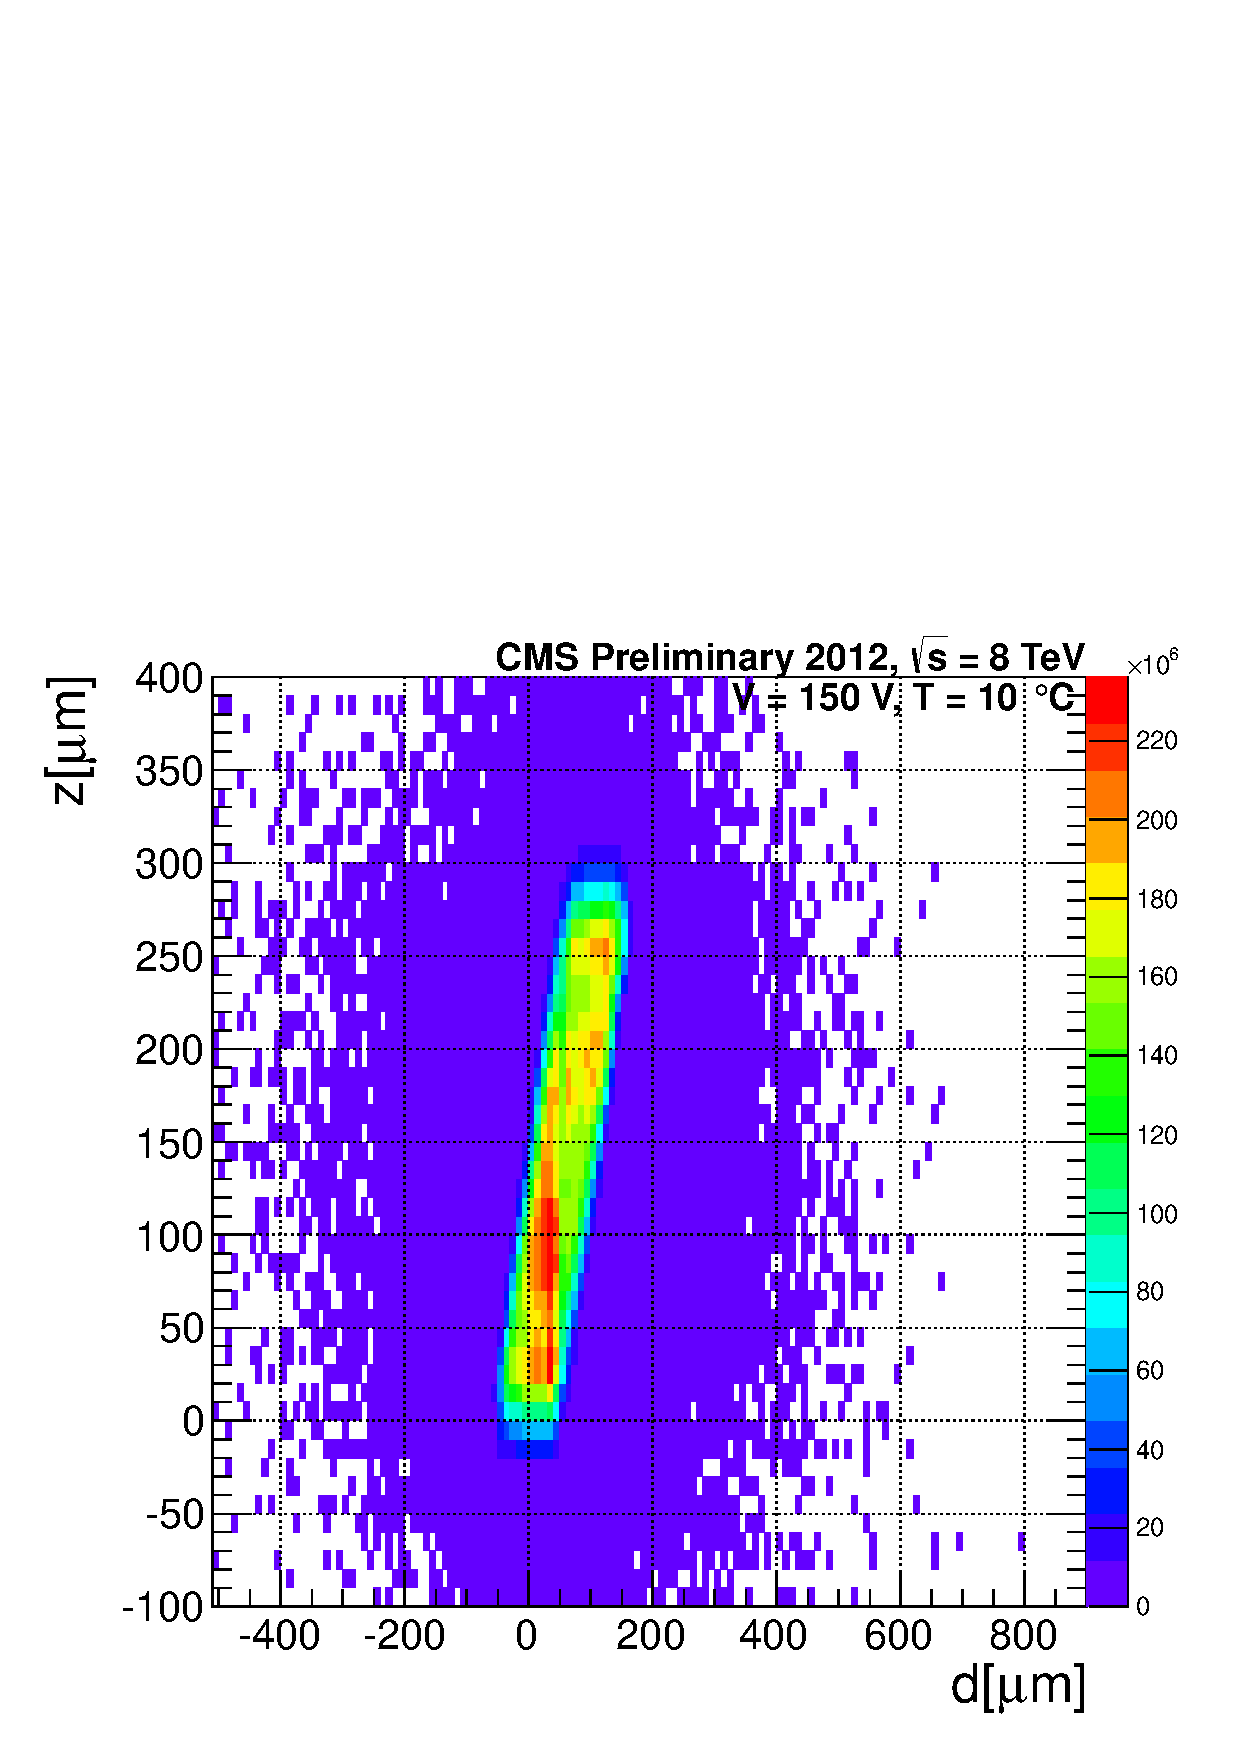
\includegraphics[width=0.5\textwidth]{Figures/LA2012_2D.png}
\caption{Depth at which electrons in silicon bulk were produced as a function of Lorentz drift.}
\label{fig:2D}
\end{figure}

\begin{figure}[ht!]
\centering
\includegraphics[width=0.5\textwidth]{Figures/LA2012_Profile.png}
\caption{The average drift of electrons as a function of the production depth. Slope of the linear fit result is the $tan \theta_L$.}
\label{fig:profile}
\end{figure}

In order to obtain a good measurement, it is important to use clean tracks. Therefore, it required to have a well reconstructed muon tracks with $p_T>3$GeV and $\chi^2/ndof<2$ which are required to have shallow impact angle with respect to local $y$ direction with cluster size of at least 4 pixels in this direction. Summary of the selection criteria can be found in table \ref{tab:sel}.

\begin{table}[ht!]
  \caption{Selection criteria for Lorentz angle measurement}
  \centering
  \begin{tabular}{l|c}
\hline
\hline
        Cluster size in y & $>3$  \\
	Track $p_t$ & $>3$GeV$/$c \\
	$\chi^2$/ndof & $<2$ \\
	Hit residuals & $<50\mu m$ \\
	Cluster charge & $<120000$e \\
\hline
\hline
  \end{tabular}
  \label{tab:sel}
\end{table}

Figure \ref{fig:La2012} shows how Lorentz angle changes with integrated luminosity. Results are shown for 23fb$^{-1}$ of delivered luminosity in 2012. Increase in Lorentz angle measured with grazing angle method has been observed in all layers, with largest effect (~6\%) visible in layer 1 over this period of data taking.  
\begin{figure}[ht!]
\centering
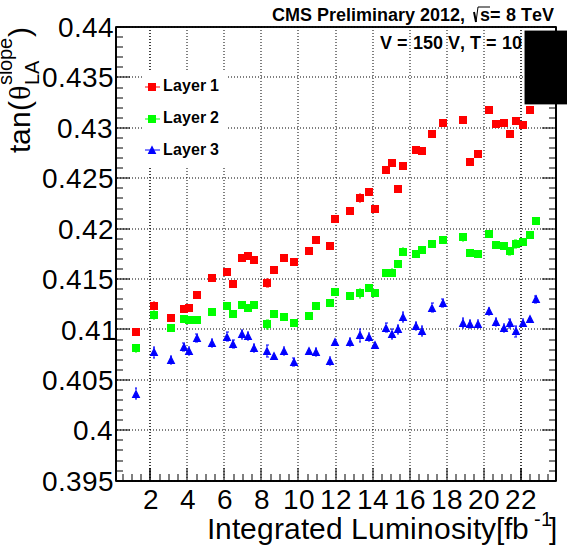
\includegraphics[width=0.5\textwidth]{Figures/LA2012.png}
\caption{Lorentz angle as a function of integrated luminosity for 2012.}
\label{fig:La2012}
\end{figure}

\section{Minimum cluster size method (V-method)}
The pixel cluster size in the drift direction depends on the incident
angle and is minimal when incident angle is equal to the Lorentz angle. Thus, measuring the average cluster size in drift direction as a function of incident angle and obtaining a minimum of that
distribution is an alternative and direct method of measuring the Lorentz angle. The method is usually referred to as V-method due
to a shape of distribution which in the simple case can be approximated with formula

\begin{equation}
p_1*abs(tan(\theta) - p_0) + p_2
\end{equation}
where $p_0$, $p_1$ and $p_2$ are parameters obtained from the fit and $p_0$ = $tan(\theta_{LA})$.

The method was successfully applied to cosmic muon tracks during CMS commissioning period in 2008 and again in 2015. The fit result is shown in figure \ref{fig:LA_VMethod}.

\begin{figure}[hbtp!]
	\centering
	\includegraphics[width=0.5\textwidth]{Figures/LA_VMethod_2015.pdf}
	\caption{An example of V-method fit.}
	\label{fig:LA_VMethod}
\end{figure}

Application to collision data is more challenging. Coordinates of a track passing through the detector, its incoming angle, and its $p_T$ are
correlated and therefore incoming angles from collision tracks have limited range. With
standard running conditions the value of Lorentz angle is at the edge of that range where tracks with very low $p_T$ ($<$0.5 GeV) dominate. Because
of that average cluster size as a function of incoming angle cannot be described by a simple model like above mentioned for cosmic data.
While  results for collision data obtained with V-method are in general agreement with the default calculation,  the uncertainty of
the method at present is too big to be used as a viable alternative.


%% Appendix Template

\chapter{Acceptance and efficiency error calculation} % Main appendix title

\label{AppendixB} % Change X to a consecutive letter; for referencing this appendix elsewhere, use \ref{AppendixX}

\lhead{Appendix B. \emph{Acceptance and efficiency error calculation}} % Change X to a consecutive letter; this is for the header on each page - perhaps a shortened title

Write your Appendix content here.
%\input{Appendices/AppendixC}

\addtocontents{toc}{\vspace{2em}} % Add a gap in the Contents, for aesthetics

\backmatter

%----------------------------------------------------------------------------------------
%	BIBLIOGRAPHY
%----------------------------------------------------------------------------------------

\label{Bibliography}

\lhead{\emph{Bibliography}} % Change the page header to say "Bibliography"

%\bibliographystyle{unsrtnat} % Use the "unsrtnat" BibTeX style for formatting the Bibliography
\bibliographystyle{unsrt}

\bibliography{Bibliography}




\end{document}
